%% Placeholder for chapter on linear equations and least squares
%%%zhipeng add the following part
%% Placeholder for chapter on linear equations and least squares




\section{Least Squares}
Consider the linear system
\begin{equation*}
Ax = y \qquad (*)
\end{equation*}
where $A\in \reals^{m\times n}$ is the coefficient data matrix (known), $y\in \reals^m$ are constraints(known) and $x\in \reals^n$ are unknown parameters that we need to figure out.

There are three possibilities for the solution of this system:

a) No $x\in \reals^n$ satisfies ($*$) 
	
b) An unique $x\in \reals^n$ satisfies ($*$) 
	
c) Many $x\in \reals^n$ satisfies ($*$) 

\vspace{0.3cm}
Since $Ax\in R(A)$, a solution $x$ will exist if $y\in R(A)$.

There is a simple test based on the ranks of augmented matrix and coefficient matrix:

1) $\rank(A) = \rank\left([A\ y] \right)$: solution to ($*$) exists

2) $\rank(A) < \rank\left([A\ y] \right)$: no solution to ($*$) exists

\vspace{0.4cm}
Suppose there exist a solution, the next question is, is it unique?

Assume a solution $\bar{x}$ exists such that $A\bar{x} = y$ (i.e., a particular solution), and there may have other solution $x$ also satisfy $Ax = y$. Therefore, we can write
\begin{align*}
Ax - A\bar{x} &= A(x -\bar{x}) = 0\\
x - \bar{x} &\in N(A)
\end{align*}

That is, any solution to ($*$) can be expressed as a sum of a particular solution plus a trival solution of, i.e.,
\begin{equation*}
x = \bar{x} + (x - \bar{x}) = \bar{x} + e
\end{equation*}
where $e\in N(A)$ (i.e., a solution to the homogeneous case $Ax = 0$).

So if there are many solutions to ($*$), we will have a affine sets given by
\begin{equation*}
\mathcal{A} = \{x|x = \bar{x} + N(A), A\bar{x} = y \}
\end{equation*}

Now, from this point of view, we could say that the solution $\bar{x}$ is unique if the elements of $N(A)$ are all zero(there is only a trival solution $e$ satisfy $Ax=0$, that is, $e$ is a zero vector), and $\bar{x}$ is any particular solution for $A\bar{x} =y$.

\vspace{0.5cm}
The three case regarding the solution of a linear system typically bread down into a question about dimensions of $A\in \reals^{m\times n}$. The results are summarized as follows
\begin{itemize}
	\item 1) Overdetermined linear system: $m>n$, more constraints than unknown parameters. Typically a solution does not exist (holds when $m$ equations are linearly independent).
	
	\item 2) Square: $m=n$, equal number of constraints and parameters, and typically there exists a unique solution.
	
	\item 3) Underdetermined linear system: $m<n$, fewer constraints than parameters, and typically many solutions exists.
\end{itemize}

\vspace{0.3cm}
\subsection{Overdetermined linear system : $m > n$ }


Assume $A$ is full column rank(i.e., full rank), $\rank(A) =n$. Therefore, $A$ is a tall and thin matrix, and $\dim(R(A)) = n < m$.

Suppose we have $m$ independent equations with $m>n$, and in this case there is no exact solution to $(*)$ (in fact this conclusion holds if there are at least $n+1$ equations are independent). This case is very commonly meet in reality, and thus we want to find a $x^*$ such that $Ax^*$ is the 'closest' to $y$, that is, to solve the following optimization problem
$$x^* = \arg \min_{x\in \reals^n}\Vert Ax - y\Vert_2$$

Note that $Ax \in R(A)$, and from the perspective of projection, we could rewrite the problem as
$$\min_{x\in \reals^{n}}||Ax - y\Vert_2 = \min_{\hat{y}\in R(A)}\Vert \hat{y} - y\Vert_2 =\prod_{R(A)}(y)$$
and this problem becomes find a projection of $y$ in the column space of $A$.

\begin{marginfigure}
	\centering
	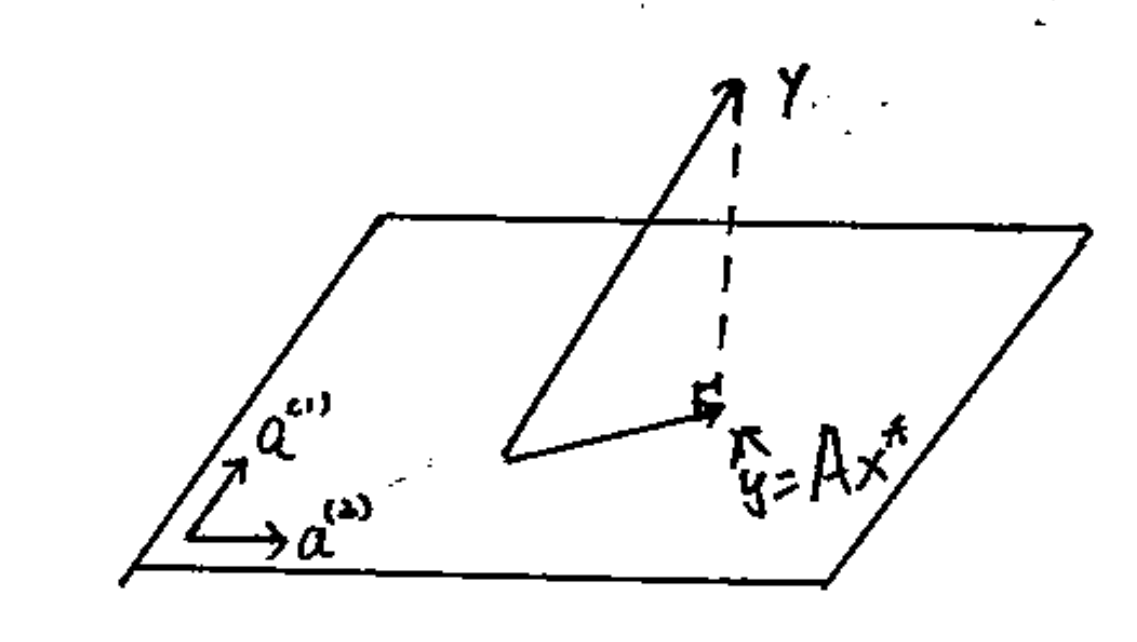
\includegraphics[width=2.1in,height=2.1in]{figures/ch06/figure1.png}
	%\caption{This is an inserted JPG graphic} 
	%\label{fig:graph} 
\end{marginfigure}

From chapter2, we know that the projection of $y$, $\hat{y}^*$, can be expressed as
\begin{equation*}
\hat{y}^* = Ax^*= \sum^n_{i=1}x_i^*a^{(i)}
\end{equation*}
where 
$A =   
\left[
\begin{matrix}
a^{(1)} & \cdots & a^{(n)}
\end{matrix}
\right]
$.

Recall what we have done before, we could solve for $x^*$ via a bunch of equations(i.e., solve for each $x_i^*$),
\begin{equation*}
\sum^n_{i=1}x_i^*\langle a^{(k)}, a^{(i)}\rangle = \langle a^{(k)}, y\rangle, \quad \forall k= 1,2,\cdots,m
\end{equation*}

For convenience, we could stack up to get what we called the normal equation:
\begin{equation*}
A^{\trans}Ax^* = A^{\trans}y
\end{equation*}

There are 2 possibilities: 

(a) $A^{\trans}A$ is invertible (this holds when $A$ has full column rank, which we have assumed in the beginning):
\begin{align*}
x^* &= (A^{\trans}A)^{-1}A^{\trans}y\\
\hat{y}^* &= A(A^{\trans}A)^{-1}A^{\trans}y
\end{align*}


(b) $A^{\trans}A$ is not invertible (if we do not assume that $A$ has full column rank):

We apply SVD to $A^{\trans}$ and  $A$:
\begin{align*}
\hat{y}^* &= A(A^{\trans}A)^{-1}A^{\trans}y\\
&= A(V
\begin{bmatrix}
\Sigma & \textbf{0}
\end{bmatrix}
\mathcal{U}^{\trans}\mathcal{U}
\begin{bmatrix}
\Sigma \\
\textbf{0}
\end{bmatrix}
V^{\trans})^{-1}A^{\trans}y\\
&= A(V\Sigma^2V^{\trans})^{-1}A^{\trans}y\\
&= AV(\Sigma^{-1})^2V^{\trans}A^{\trans}y\\
&= \mathcal{U}
\begin{bmatrix}
\Sigma \\
\textbf{0}
\end{bmatrix}
V^{\trans}V\Sigma^{-2}V^{\trans}V
\begin{bmatrix}
\Sigma & \textbf{0}
\end{bmatrix}
\mathcal{U}^{\trans}y\\
&= \mathcal{U}
\begin{bmatrix}
\Sigma \\
\textbf{0}
\end{bmatrix}
\Sigma^{-1}\Sigma^{-1}
\begin{bmatrix}
\Sigma & \textbf{0}
\end{bmatrix}
\mathcal{U}^{\trans}y\\
&= \mathcal{U}
\begin{bmatrix}
I_r\\
\textbf{0}
\end{bmatrix}
\begin{bmatrix}
I_r & \textbf{0}
\end{bmatrix}
\mathcal{U}^{\trans}y\\
&= \mathcal{U}
\begin{bmatrix}
I_r& \textbf{0}\\
\textbf{0} & \textbf{0}
\end{bmatrix}
\mathcal{U}^{\trans}y\\
&= \mathcal{U}
\begin{bmatrix}
I_r& \textbf{0}\\
\textbf{0} &  \textbf{0}
\end{bmatrix}
\begin{bmatrix}
\langle u^{(1)}, y\rangle\\
\langle u^{(2)}, y\rangle \\
\vdots\\
\langle u^{(m)}, y\rangle
\end{bmatrix}\\
&= \sum^r_{i=1}\langle u^{(i)}, y\rangle u^{(i)}
\end{align*}


\subsection{Uniquely determined: $m =n$}
Given the linear system with $m=n$
$$Ax = y$$

The solution is given by
$$x^* = A^{-1}y$$

Note that:

(a) There are equal number of constraints and parameters in this case.

(b) We assume that $A$ has full rank (both columns and rows).
	
(c) Since $A$ is a square matrix with full rank, $A^{-1}$ exists.



\subsection{Underdetermined linear system: $m<n$ }

Note that

	(a) Since $m<n$, $A$ is a wide and short matrix.
	
	(b) In this case, there are more parameters than constraints.
	
	(c) We assume that $A$ has full row rank, so $\rank(A) = m$
	
	(d) Hence, there are many solutions.

\vspace{0.3cm}

Since in this case, there are many solutions satisfy the linear equation $Ax=y$, then the idea to pick the optimal one is, we choose a solution $x$  with the shortest length in the sense of $L_2$ norm, that is, solve the following optimization problem
$$x^* = \arg  \min_{Ax = y, x\in \reals^n}\Vert x\Vert _2$$

Alternatively, we can rephrase the problem from the perspective of projection
\begin{equation*}
\min_{Ax = y, x\in \reals^n}\Vert x\Vert  = \min_{x\in \reals^n, x\in \mathcal{A}}\Vert x - 0\Vert  = \prod_{\mathcal{A}}(0)
\end{equation*}
since the set $\{x | Ax= y \}$ is an affine space. Therefore, the problem becomes finding the projection of origin from the affine space $\mathcal{A}$.



\begin{figure}
	\centering
	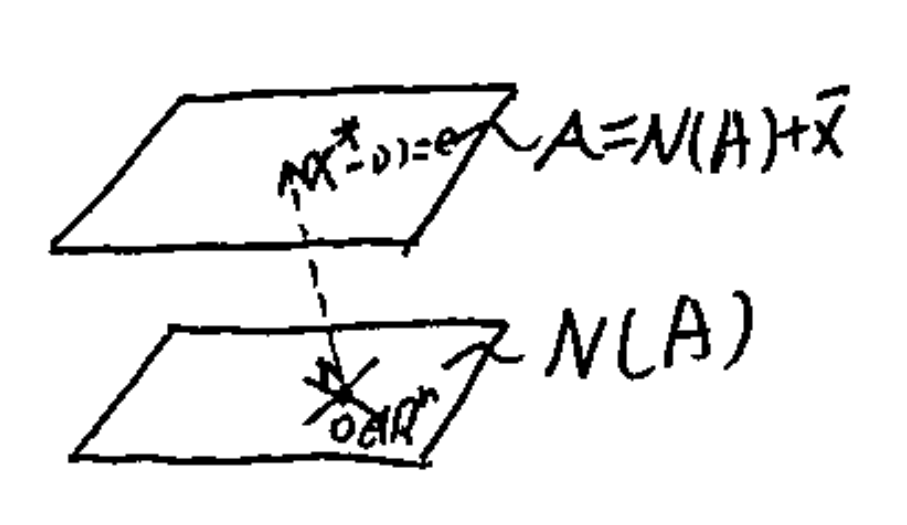
\includegraphics[width=1.6in,height=1.6in]{figures/ch06/figure3.png}
	%\caption{This is an inserted JPG graphic} 
	%\label{fig:graph} 
\end{figure}

To solve for $x^*$, note (from before) error vector 
\begin{align*}
e &= x^* - 0 = x^* \perp N(A)\\
x^* &\in N(A)^{\perp} = R(A^{\trans})
\end{align*}

So we can write $x^* = A^{\trans}\alpha$ for some $\alpha \in \reals^m$. For $x^*$ to be in $\mathcal{A}$ it must satisfy that $Ax^* = y$, substituting in we get 
\begin{equation*}
Ax^* = y= AA^{\trans}\alpha
\end{equation*}

By assumption, $A$ is full row rank so $AA^{\trans}$ is invertible, so 
$$\alpha = (AA^{\trans})^{-1}y$$

and the optimal solution is given by
$$x^* = A^{\trans} \alpha = A^{\trans}(AA^{\trans})^{-1}y$$

In addition, $A^{+} =A^{\trans}(AA^{\trans})^{-1}$ is  what we called the Moore–Penrose pseudo inverse of $A$ (and it is also the right inverse of $A$ provided $A$ has full row rank).

Furthermore, we apply SVD to $A$ and $A^{\trans}$,
\begin{align*}
x^* &= A^{\trans}(AA^{\trans})^{-1}y\\
&= A^{\trans}\left[\mathcal{U}
\begin{bmatrix}
\Sigma & \mathbf{0}
\end{bmatrix}
V^{\trans}V
\begin{bmatrix}
\Sigma\\
\mathbf{0}
\end{bmatrix}
\mathcal{U}^{\trans}\right]^{-1}y\\
&= A^{\trans}(\mathcal{U}\Sigma^2\mathcal{U}^{\trans})^{-1}y\\
&= A^{\trans}\mathcal{U}\Sigma^{-2}\mathcal{U}^{\trans}y\\
&= V
\begin{bmatrix}
\Sigma\\
\mathbf{0}
\end{bmatrix}
\mathcal{U}^{\trans}\mathcal{U}\Sigma^{-2}\mathcal{U}^{\trans}y\\
&=V
\begin{bmatrix}
\Sigma^{-1} \\
\mathbf{0}
\end{bmatrix}
\mathcal{U}^{\trans}y\\
&= V
\begin{bmatrix}
\Sigma^{-1}\\
\mathbf{0}
\end{bmatrix}
\begin{bmatrix}
\langle u^{(1)}, y\rangle\\
\vdots\\
\langle u^{(n)}, y\rangle
\end{bmatrix}\\
&= \sum^r_{i=1}\frac{1}{\sigma_i}\langle u^{(i)}, y\rangle v^{(i)}
\end{align*}





\vspace{0.3cm}
\subsection{Interpretation of $x^*= \arg \min_x \Vert y-Ax\Vert_2$}


\quad\ (1). Approximated solution to $y=Ax$

$y^*=Ax^*$ is the 'best' approximated solution in the sense of $L_2$ norm, which means, $y^*$ is the closest point in $R(A)$ to $y$.

(2). Minimum perturbation of $y$ to 'feasibility'

\begin{figure}
	\centering
	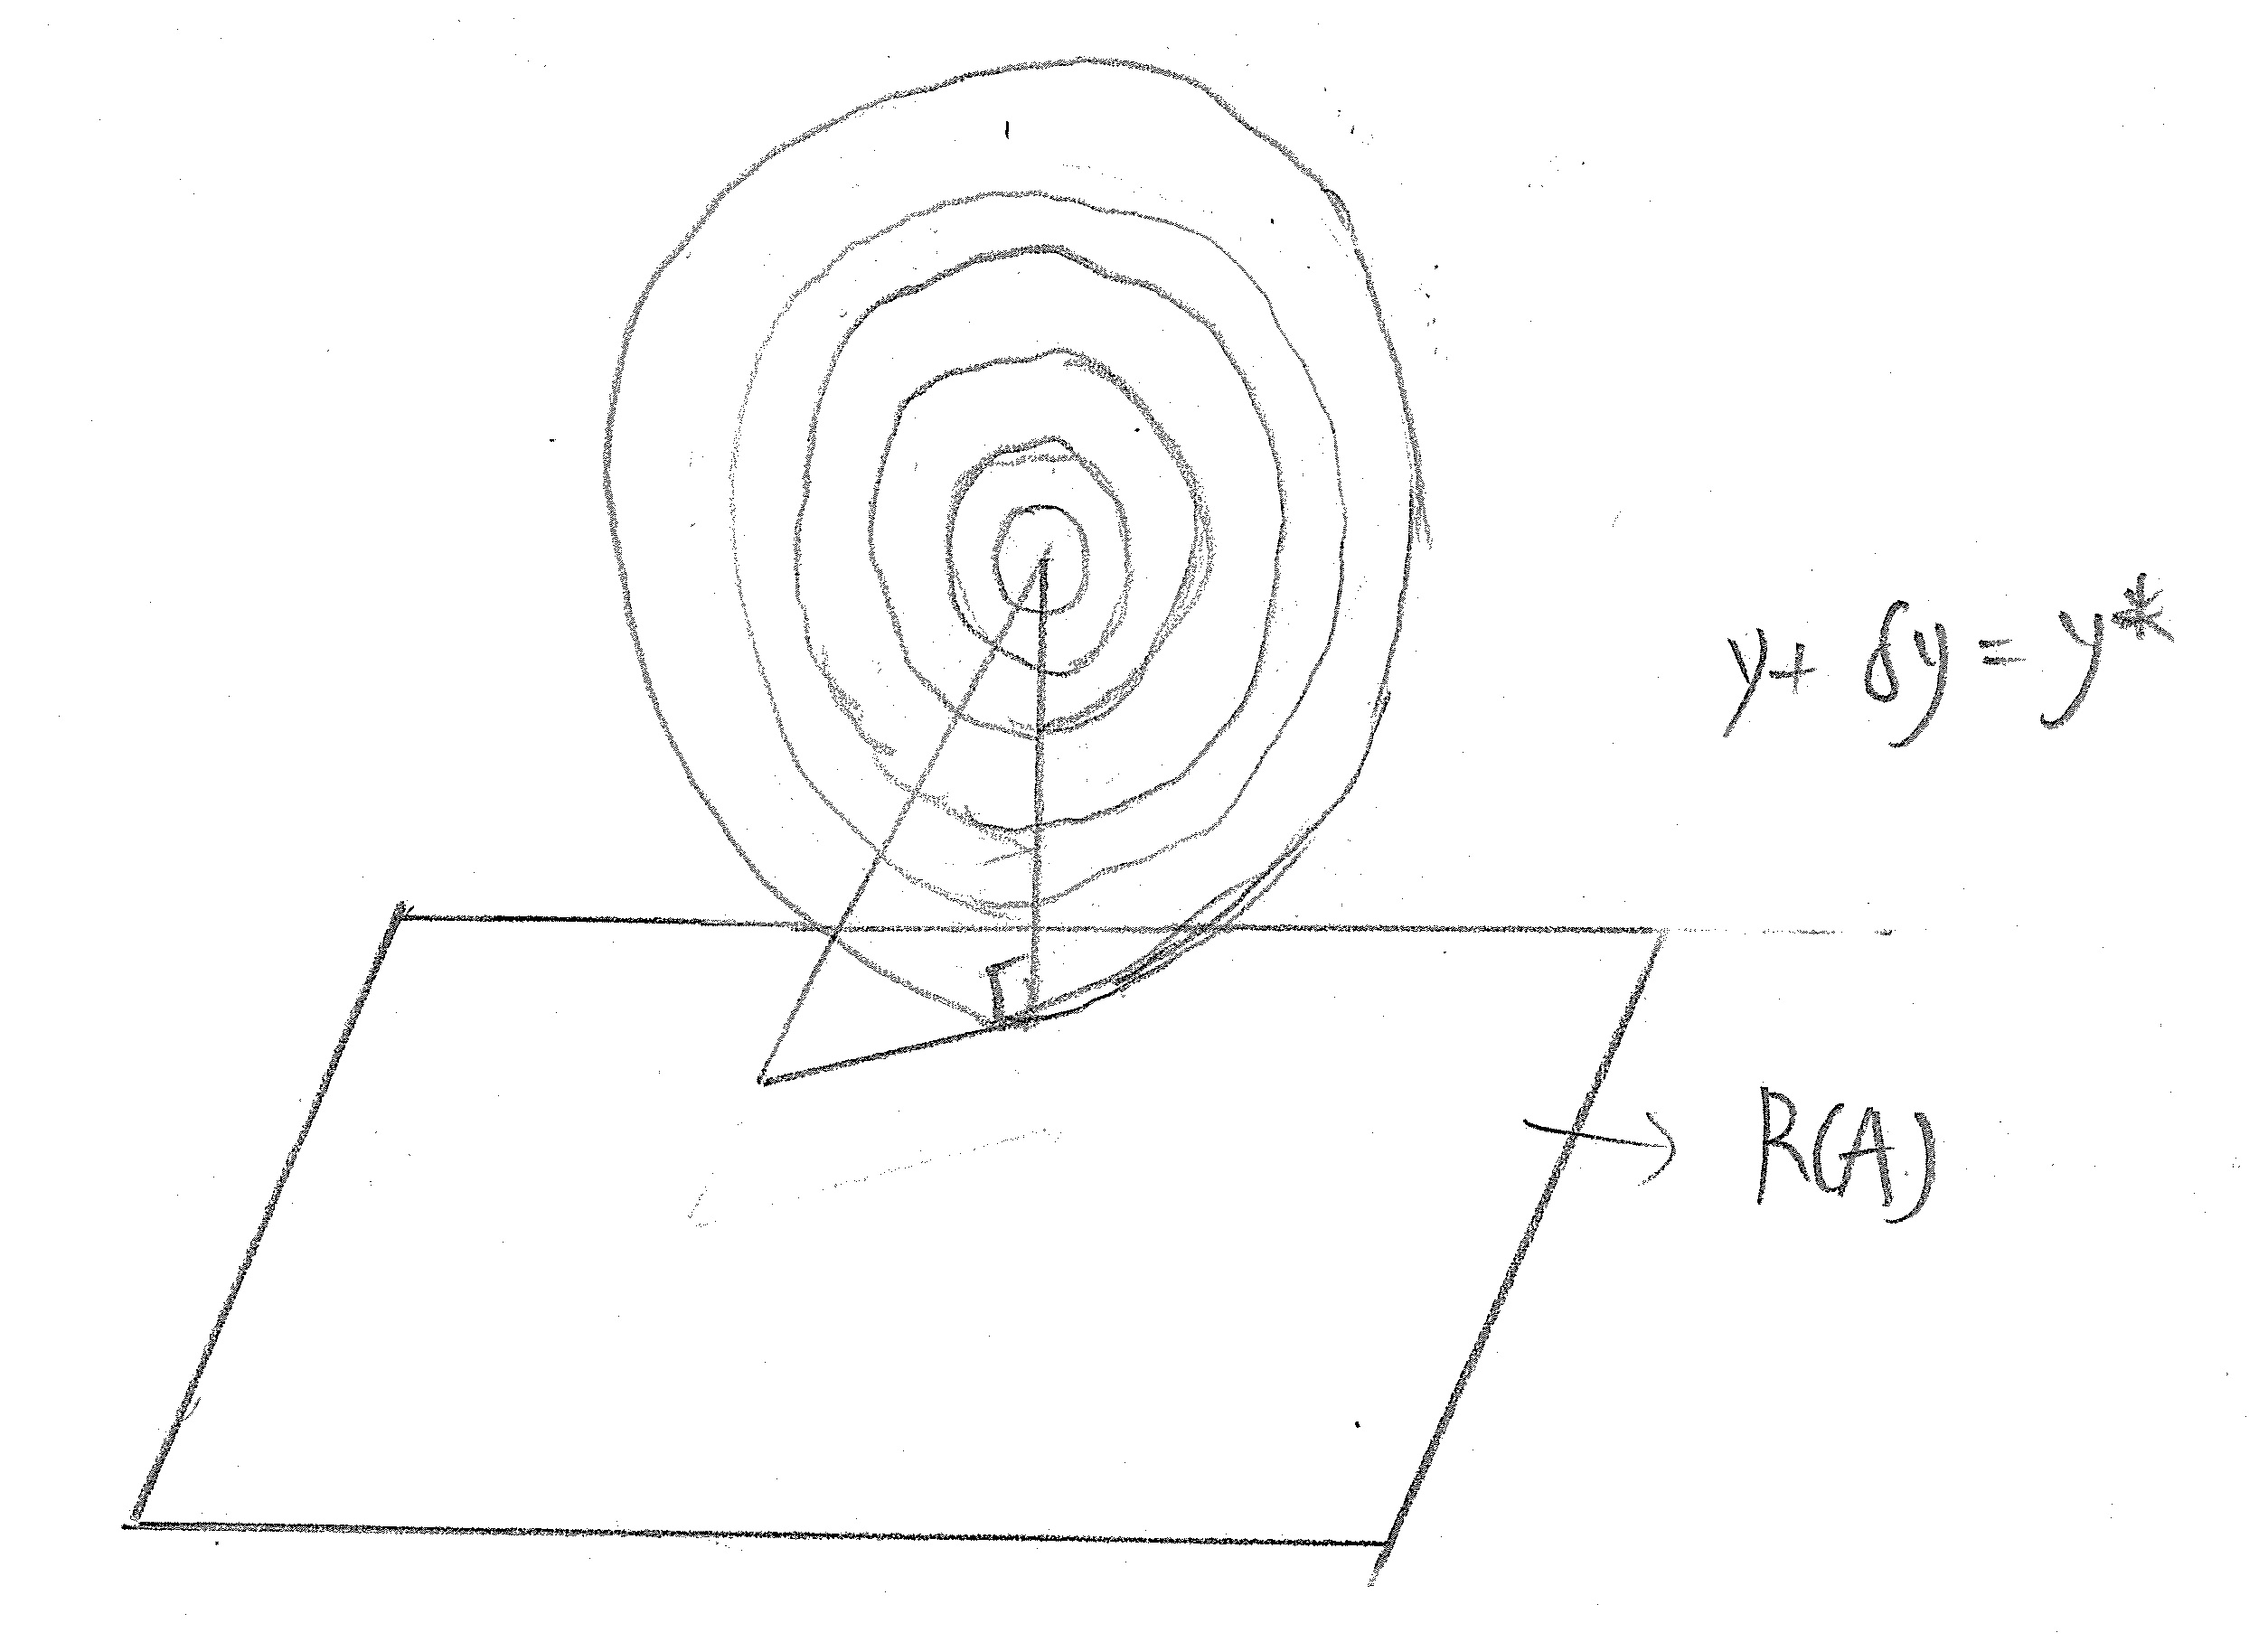
\includegraphics[width=2in,height=2in]{figures/ch06/ch06-01.jpg}
	%\caption{This is an inserted JPG graphic} 
	%\label{fig:graph} 
\end{figure}

(3). Perturb both $y$ and $A$ to get 'feasibility'

"Total least square"

Suppose there are only pertubation for $y$ but also pertubation of $A$, formally we want to solve the following optimization problem
\begin{align*}
\min_{\delta y,  \delta A} & \left\Vert [\delta A\ \delta y] \right\Vert_F \\
s.t.\quad& y +\delta y = (A + \delta A) x
\end{align*}
where $\delta A\in \reals^{m\times n}$, $\delta y \in\reals^m$,  and also $[\delta A\ \delta y]$ is a $m$ by $n+1$ matrix, $y+\delta y\in R(A+\delta A)$. To solve this problem, we may utilize SVD.


(4). Linear regression
$$\Vert y-Ax\Vert ^2_2 = \sum_{i=1}^{m} ( y_i - \langle a^{(i)} , x\rangle )^2 = \sum_{i=1}^{m} r_i^2$$
where $r_i$ defined as the residual, and thus the standard least square problem can also be interpreted as a problem of minimizing the sum of square of residuals.

\begin{figure}
	\centering
	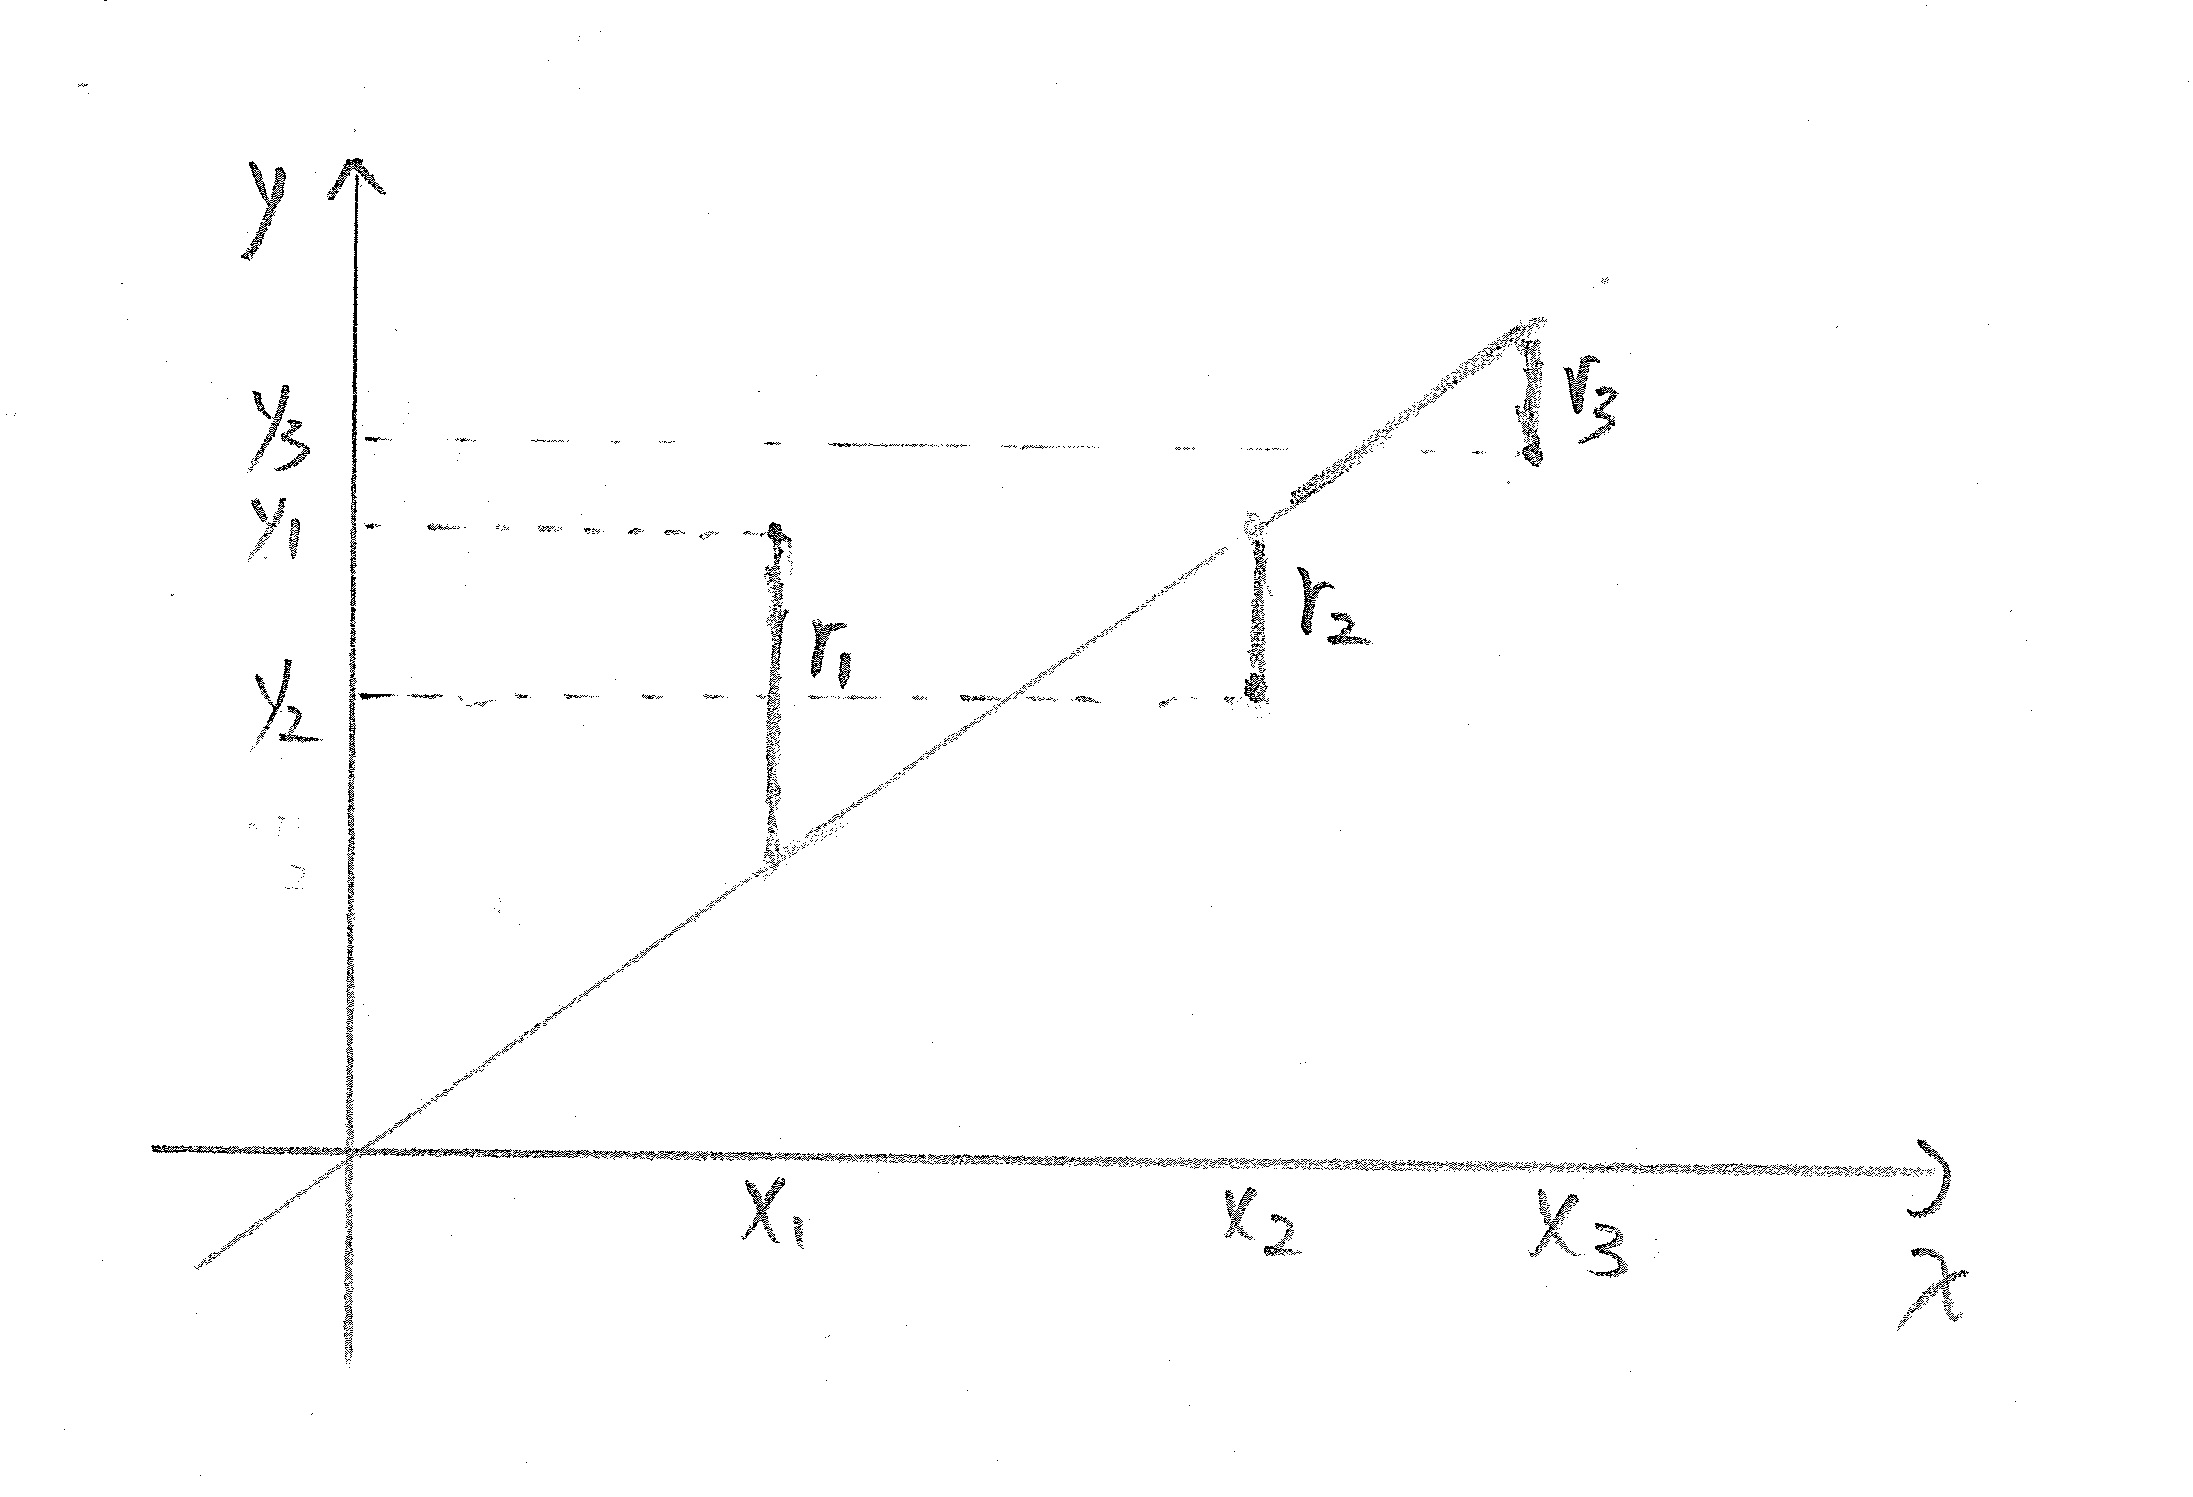
\includegraphics[width=2in,height=2in]{figures/ch06/ch06-02.jpg}
	%\caption{This is an inserted JPG graphic} 
	%\label{fig:graph} 
\end{figure}


\begin{example}

Let's consider fitting a line to $\{(0,6),(1,0),(2,0) \}={(a_i,y_i)}.$

The approximation takes the form of $y=x_1+ax_2$, and we want to choose a vector $x$ to minimize $\sum_{i=1}[y_i-(x_1+a_ix_2)]^2 = \sum_{i=1} r_i^2$, that is, we want to minimize the following
\begin{align*}
\Vert y- Ax\Vert_2^2 
&=
\left\Vert
\begin{bmatrix}
6\\
0\\
0
\end{bmatrix}
-
\begin{bmatrix}
1&0\\
1&1\\
1&2
\end{bmatrix}
\begin{bmatrix}
x_1\\
x_2
\end{bmatrix}
\right\Vert_2^2\\
&=\Vert y-Ax^*\Vert^2_2\\
&=6
\end{align*}

To solve for $x^*$, we have
$x^*=(A^{\trans}A)^{-1}A^{\trans}y=[5 , -3]^{\trans}$

Thus, the equation for this line is
$$\hat{y}^*=x_1^*+ax_2^*=5-3a$$            %so x1 and x2 are parameters

This example also illustrates that, if we would like to add an intercept term in the linear model, we could just let the first column of $A$ be an vector will all entries are $1$.
\end{example}


\section{Variants of least square}

\subsection{Weighted least square}
In the previous classical least square method, we do not consider the weights for each square of the residual(i.e., all of them are equally weighted), however, some residuals might be more important than the others. A very natural approach is to assign different weights to different $r_i^2$.

Formally, we formulate the optimization problem as
\begin{align*}
\min \sum_{i=1}^{n} w_i^2 r_i^2
&=\Vert W (y-Ax)\Vert ^2_2\\
&=\Vert Wy-WAx)\Vert ^2_2\\
&=\Vert \bar{y}-\bar{A}x \Vert ^2_2
\end{align*}
where $W=\diag(w_1, w_2, \cdots, w_m)$ and each $w_i\geq 0$, $\bar{y} \triangleq Wy$ and $\bar{A} \triangleq WA$. 

From the last two equities, we may find that this is very similar with the classic one but now we need to solve for $x$ in a transformed coordinate system.

To solve for $x^*$, we analogy to the solution of standard least square, and we have the normal equation
$$\bar{A}^{\trans} \bar{A} x=\bar{A}^{\trans} \bar{y}$$
so the solution is given by
$$x^*=(A^{\trans} W^{\trans} W A)^{-1} A^{\trans} W^{\trans} W y$$


In fact, if $W$ is positive definite(and thus $W^T W$ is positive definite), we can use a more general transform with PD, 
$$\Vert W (y-Ax)\Vert ^2_2 = (y-Ax)^{\trans}W^{\trans}W(y-Ax)=r^{\trans}W^{\trans}Wr$$
where $r$ is the residual in the original coordinate system, and we recognize that this objective is indeed an ellipsoid.

\newpage
\vspace{0.3cm}
Standard LS
\begin{figure}
	\centering
	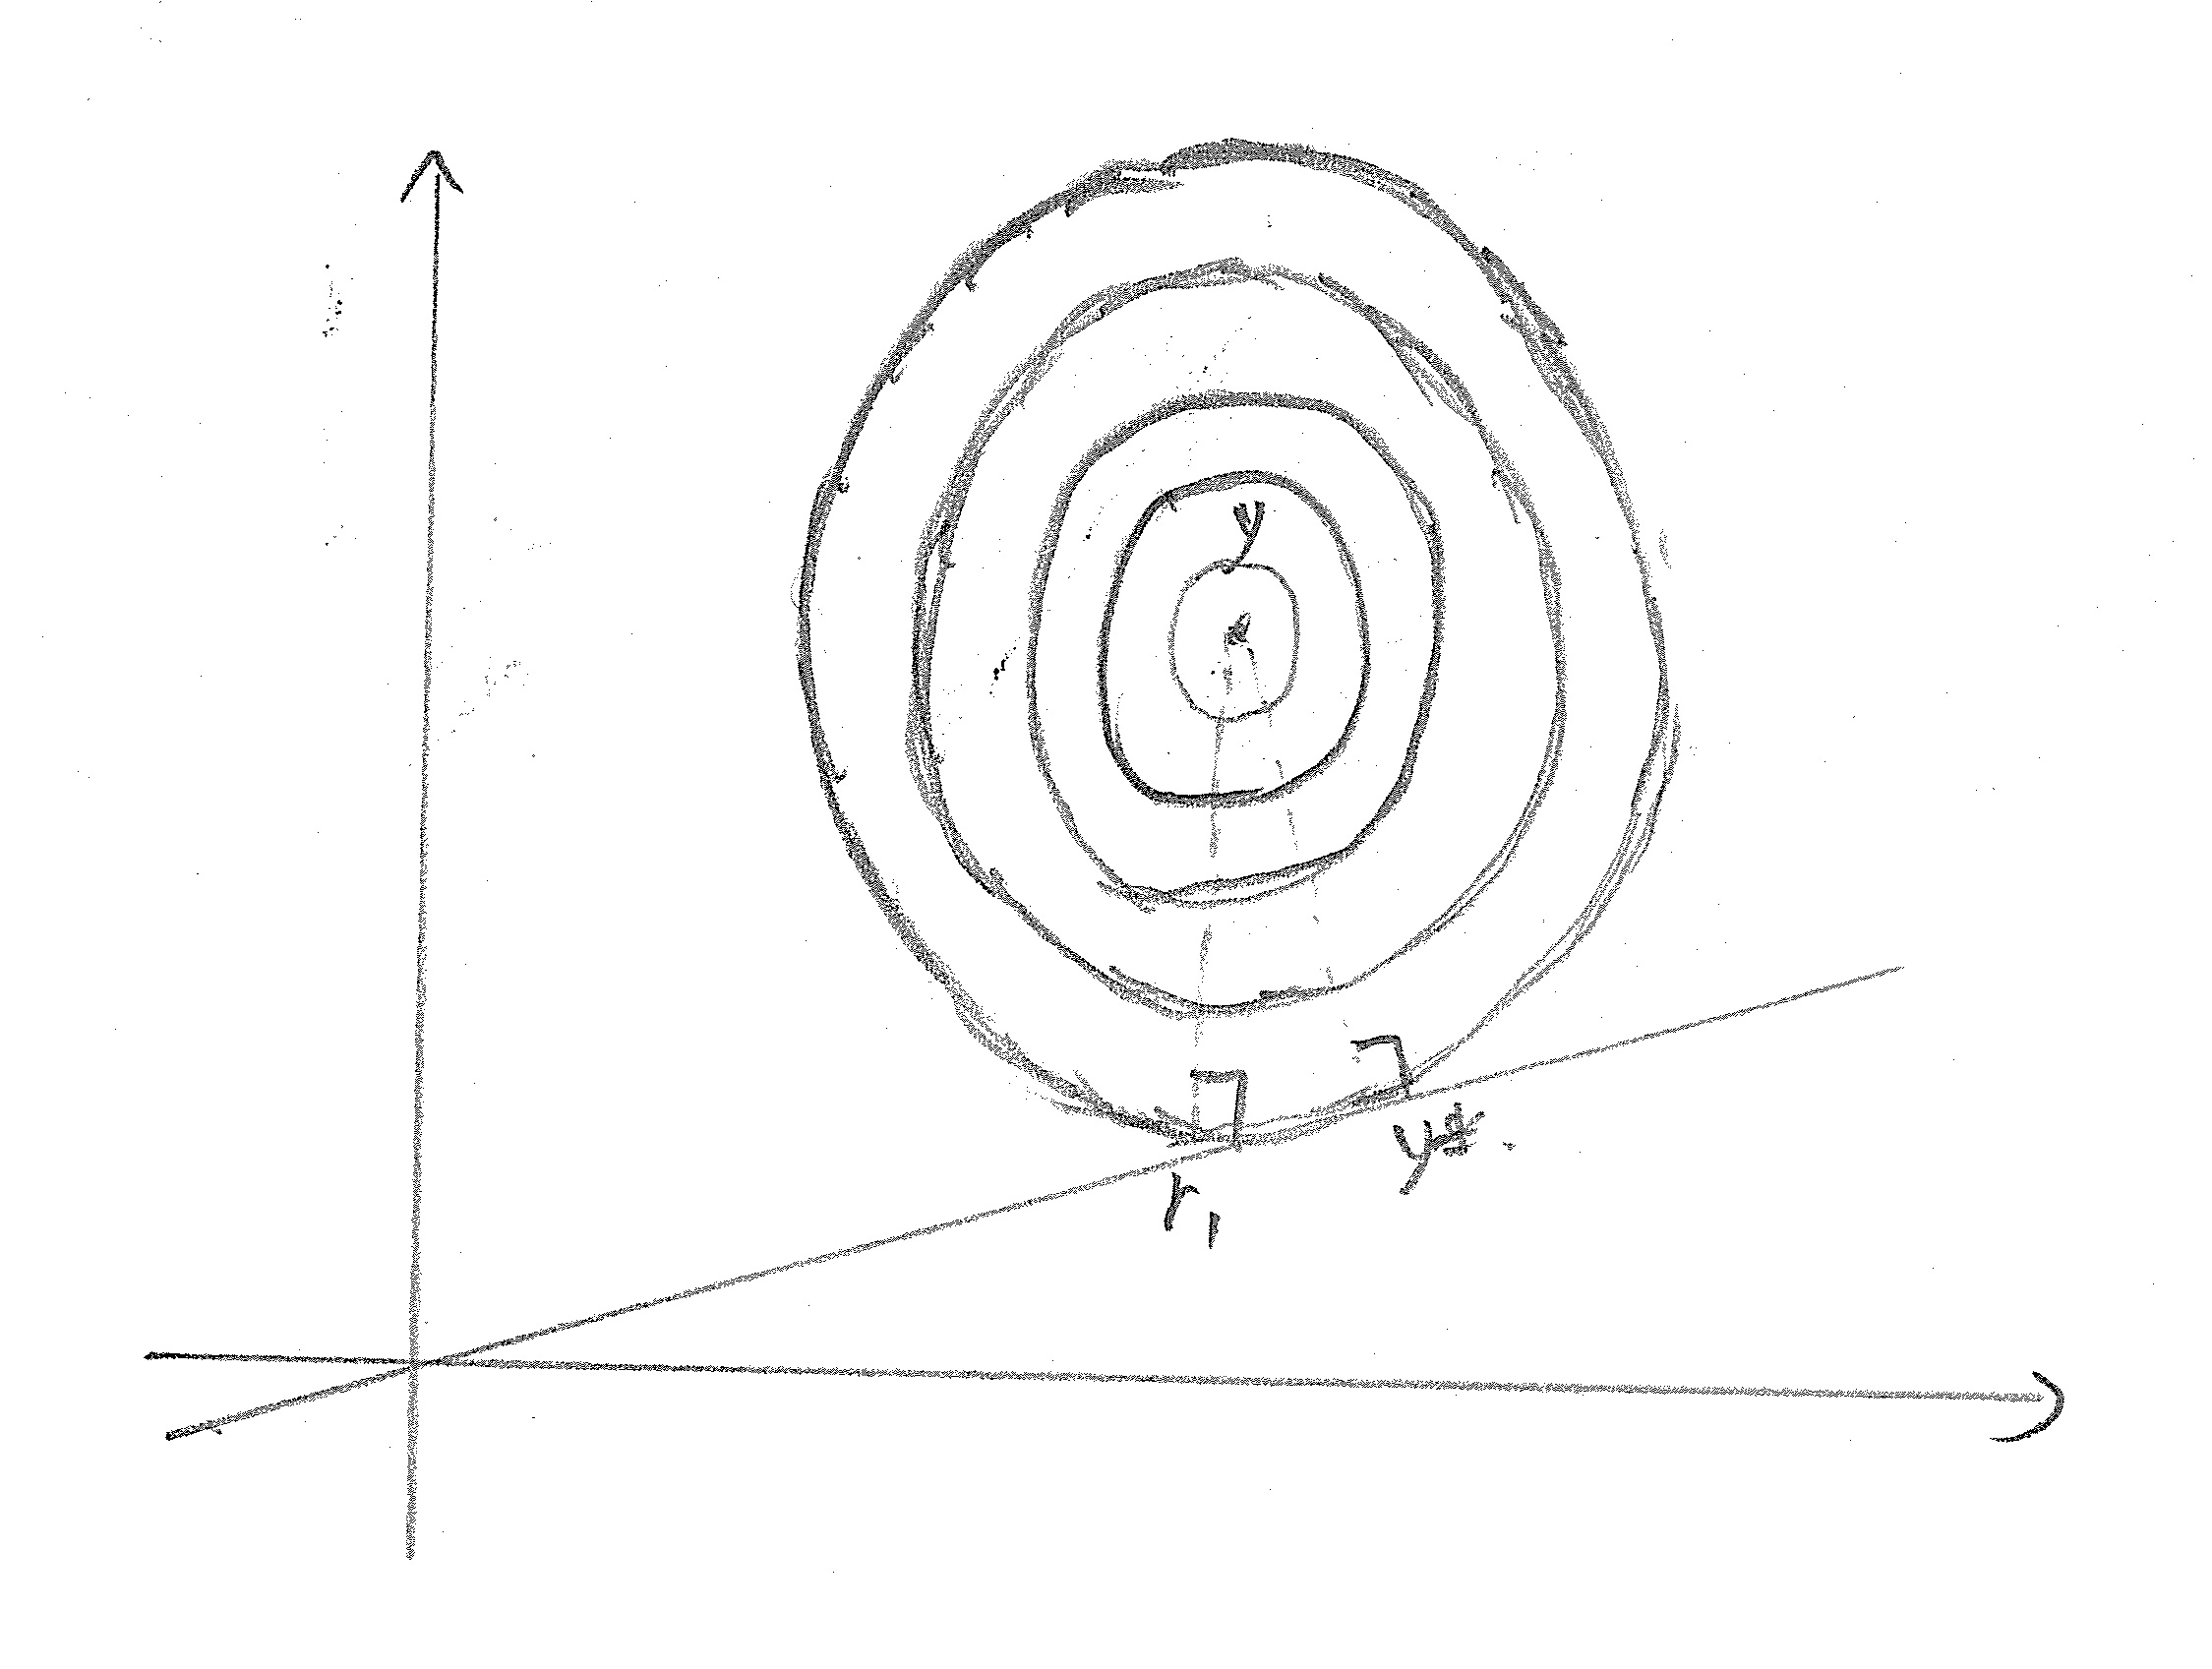
\includegraphics[width=2in,height=2in]{figures/ch06/ch06-03.jpg}
	%\caption{This is an inserted JPG graphic} 
	%\label{fig:graph} 
\end{figure}

Weighted LS with $W$ is diagonal 

\begin{figure}
	\centering
	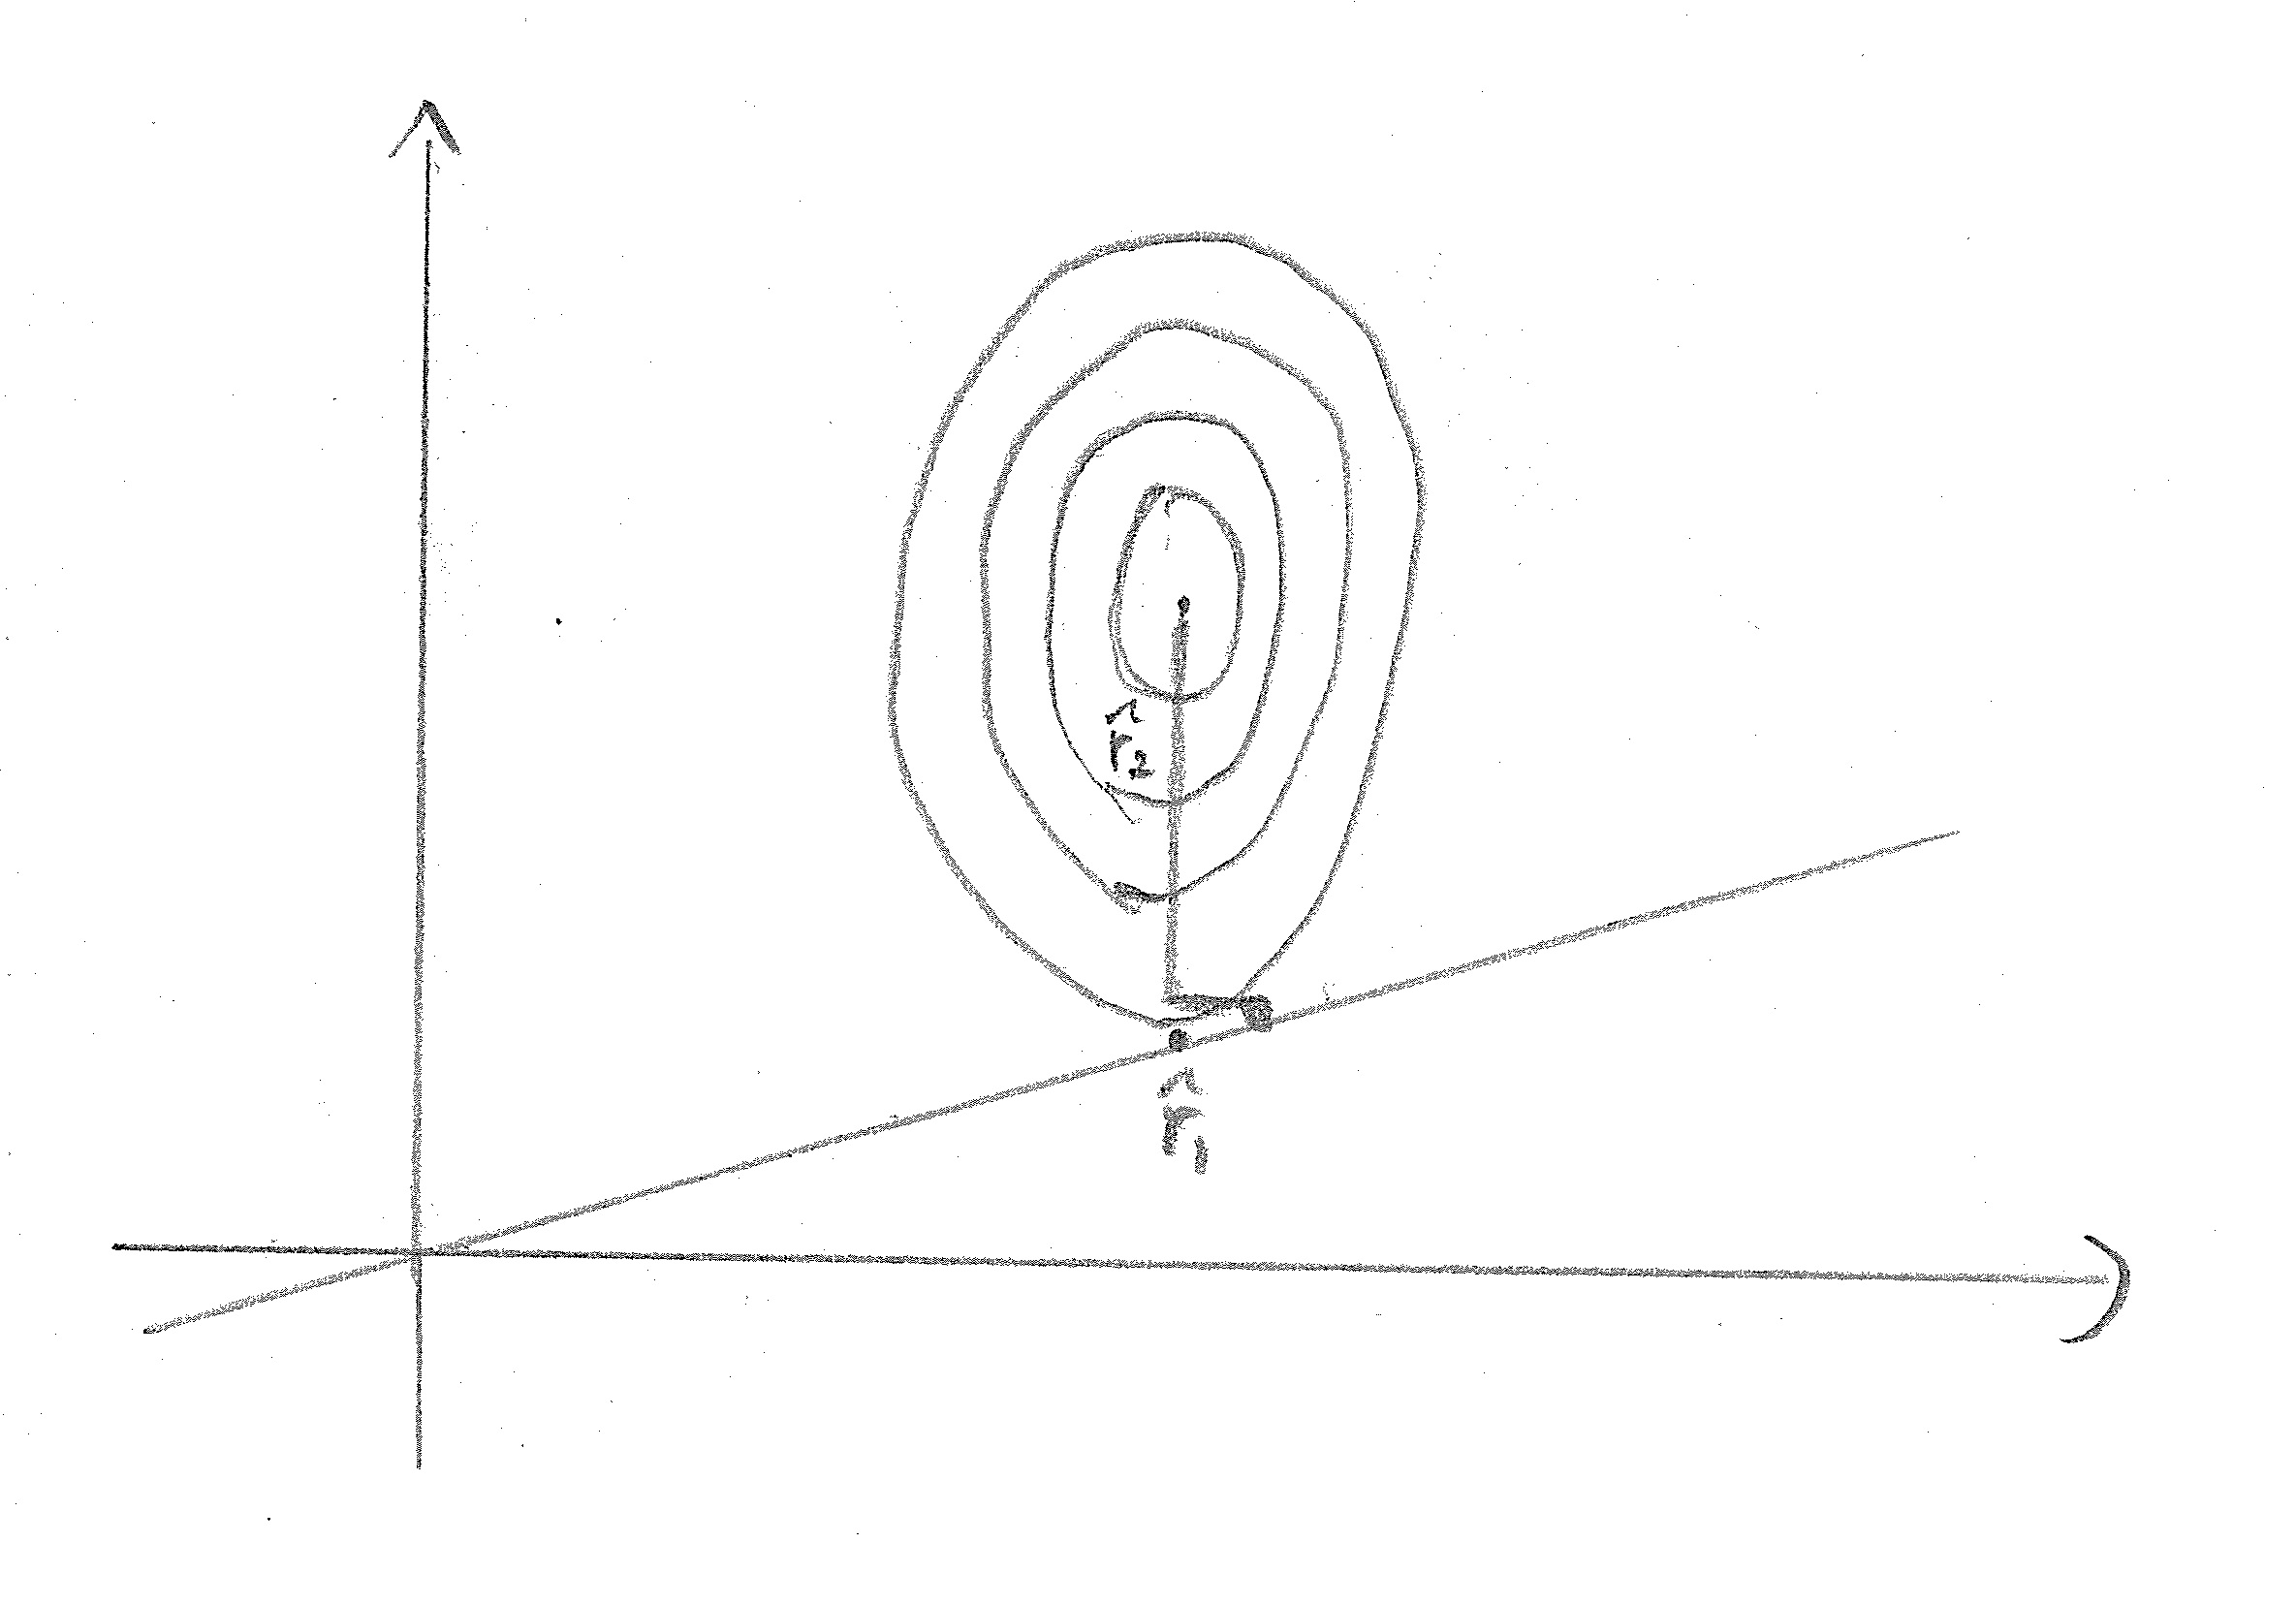
\includegraphics[width=2in,height=2in]{figures/ch06/ch06-04.jpg}
	%\caption{This is an inserted JPG graphic} 
	%\label{fig:graph} 
\end{figure}

Weighted LS with $W$ is PSD (rotation)

\begin{figure}
	\centering
	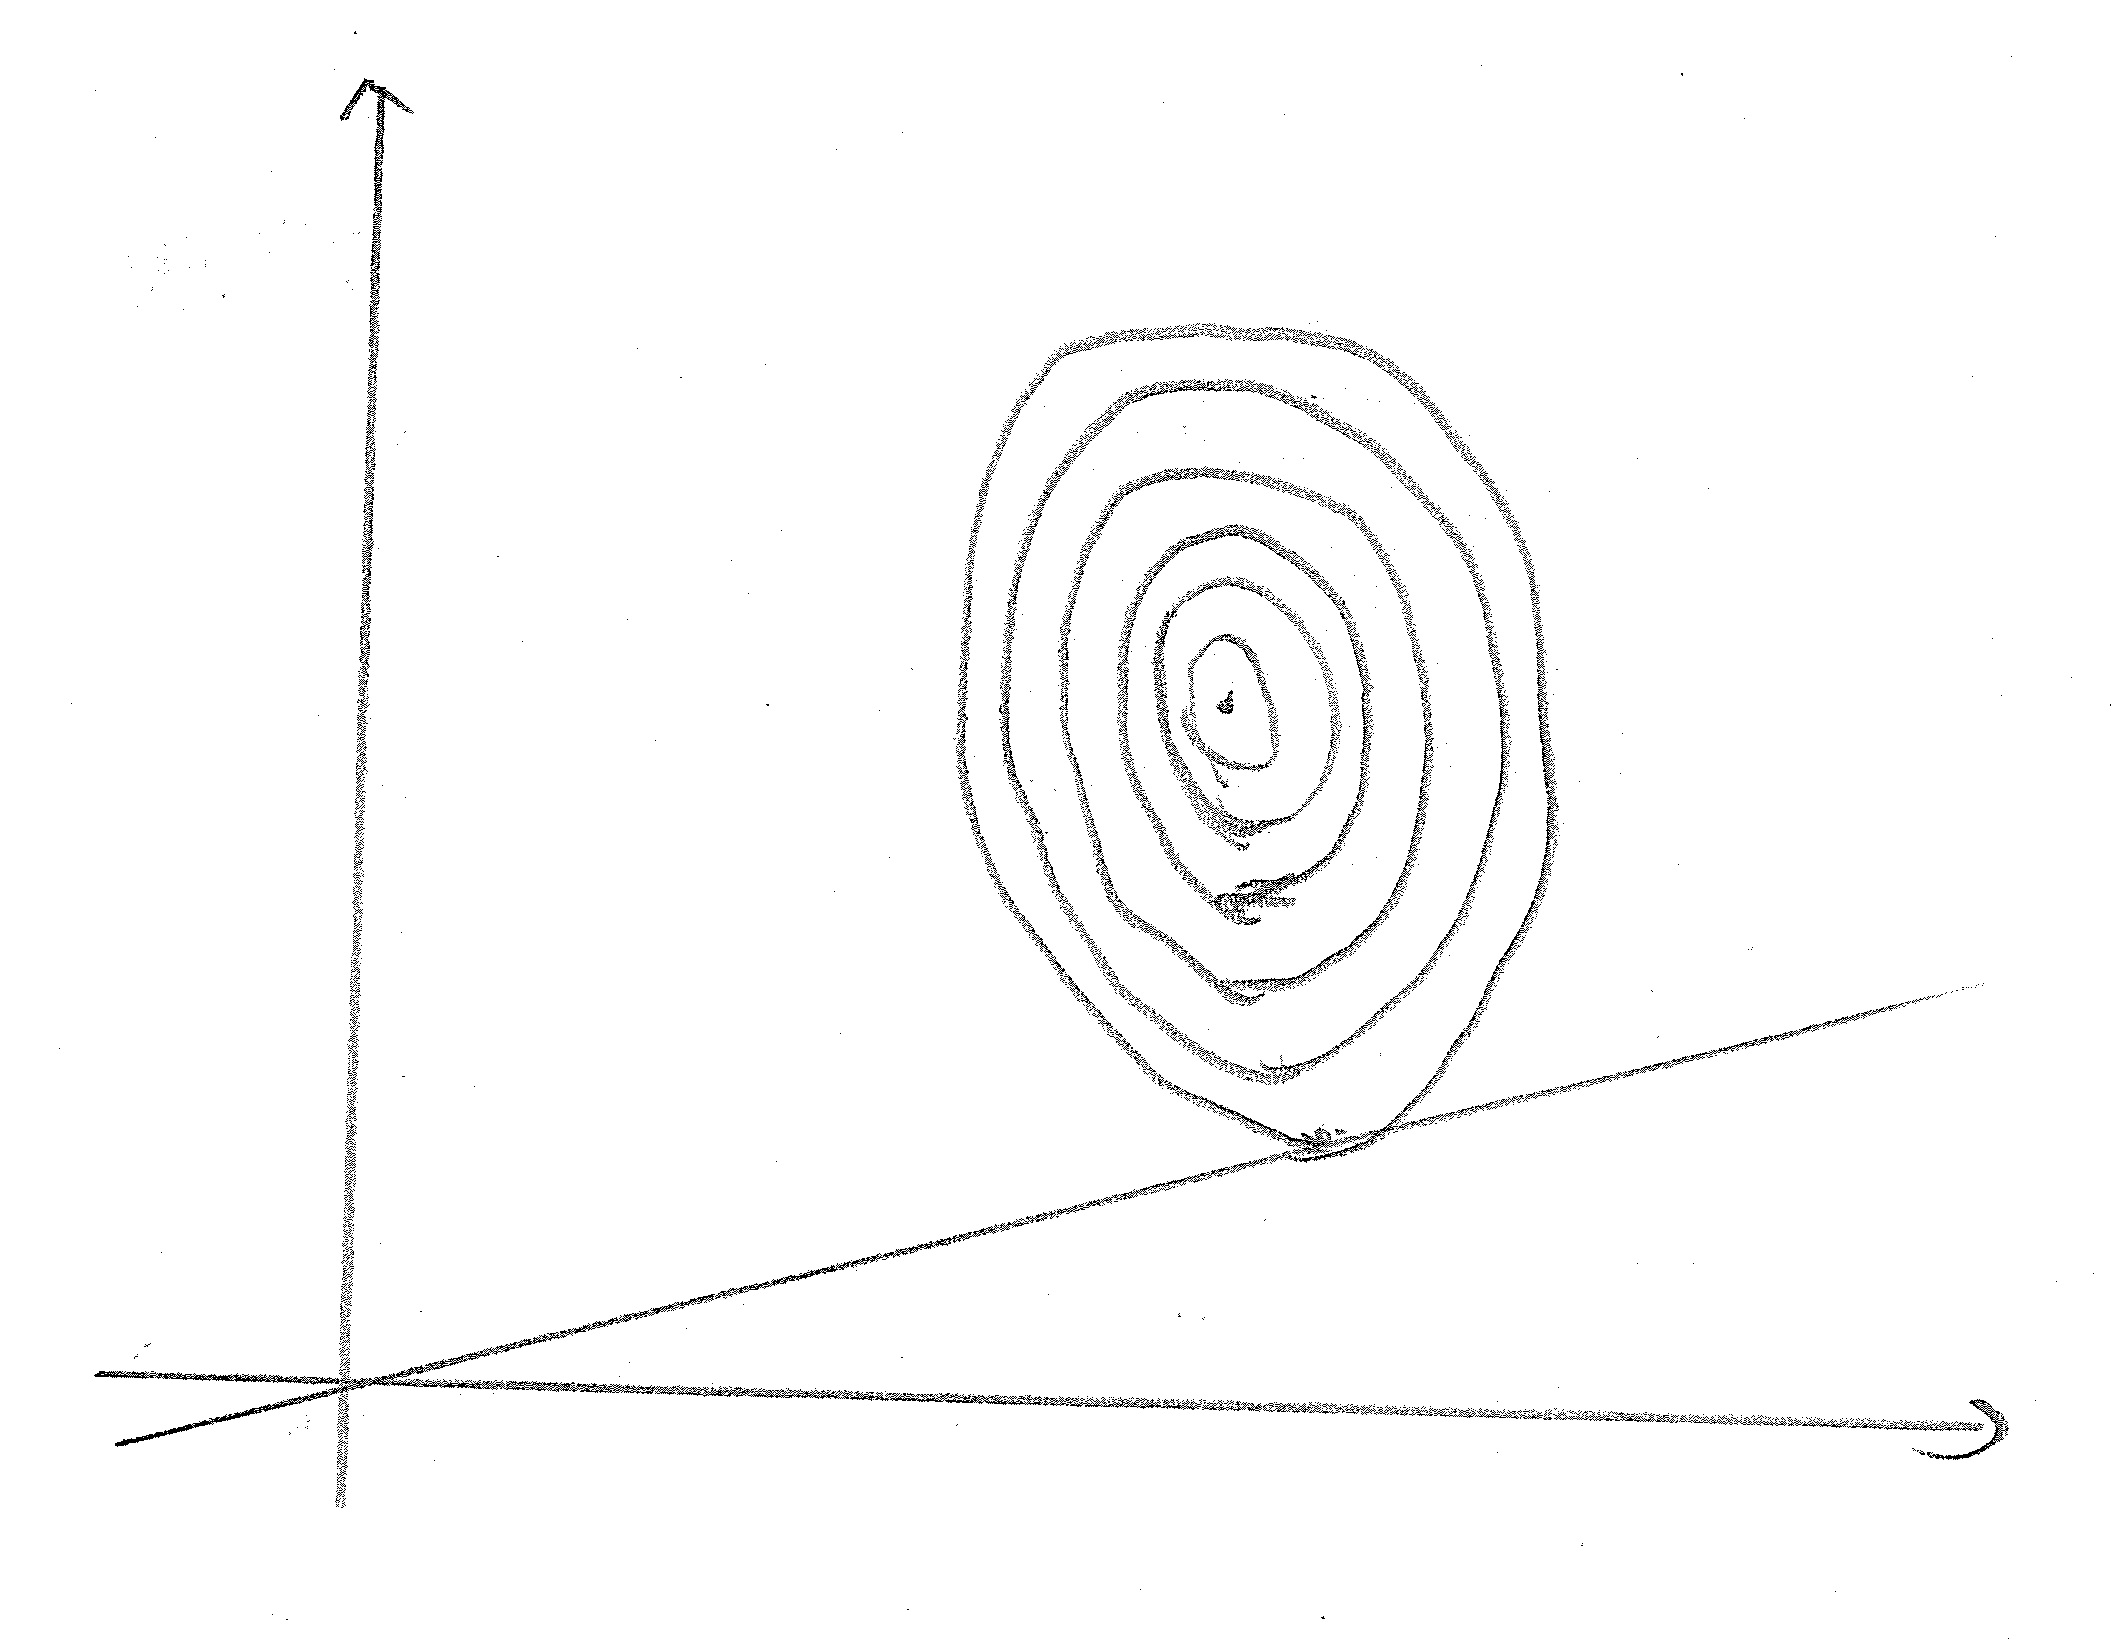
\includegraphics[width=2in,height=2in]{figures/ch06/ch06-05.jpg}
	%\caption{This is an inserted JPG graphic} 
	%\label{fig:graph} 
\end{figure}



\subsection{$L_2$- regularization least square}

In the standard least square, we do not have preference for any specific $x$ over any other, and often $x$ is a vector of resources consumed.


The $L_2$ regularized least square problem is formulated as
$$x^*=\arg_{x\in\reals_{n}} \min \Vert y-Ax\Vert ^2_2 + \gamma \Vert x\Vert ^2_2$$
where $\gamma\geq 0$ is a scalar (so if $\gamma = 0$ we retrieve the standard LS), and the term $\gamma \Vert x\Vert ^2_2$ is called the regularization or penalty term.


To solve regularized least square, we first recall a basic result regarding the $L_2$ norm, for any vectors $a$ and $b$, we have
$$\left\Vert 
\begin{bmatrix}
a\\
b
\end{bmatrix}
\right\Vert_2^2
=\Vert a \Vert_2^2 + \Vert b \Vert_2^2$$

With this useful result(can be proved easily by utilizing the definition of $L_2$ norm), we could rewrite the objective function by first define
$$
\bar{A}=
\begin{bmatrix}
A\\
\sqrt{\gamma} I_n
\end{bmatrix}
,
\bar{y}=
\begin{bmatrix}
y\\
0_n
\end{bmatrix}
$$
and therefore the objective can be written as
$$\Vert Ax - y\Vert ^2_2 + \gamma \Vert x\Vert ^2_2=\Vert \bar{A}x-\bar{y}\Vert^2_2$$

Similar with the standard least square, we can solve for $x^*$ by the following
$$x^*=(\bar{A}^{\trans} \bar{A})^{-1} \bar{A}^{\trans} \bar{y}=(A^{\trans} A+\gamma I)^{-1} A^{\trans} y$$

\subsection{Tikhonov regularization(ridge regression)}
A more general format for regularized LS allows for the introduction of weighting matrices on the
output matching residuals and on the deviation of the input term from a nominal value, resulting in the following generalize regularized problem,
$$\min_x \Vert W_1 (Ax - y)\Vert^2_2 + \Vert W_2 (x - x^{(0)})\Vert^2_2 = \min_x \Vert \bar{A}x-\bar{y}\Vert^2_2 $$
where $\bar{A} := 
\begin{bmatrix}
W_1 A\\
W_2
\end{bmatrix}
,
\bar{y} := 
\begin{bmatrix}
	W_1 y\\
	W_2 x^{(0)}
\end{bmatrix}
$
, and $W_1$ and $W_2$ are PD.

Clearly, this is a special case of our previous $L_2$ regularization, with $W_1 = I_m$, $W_2 = \sqrt{\gamma} I_n$, $x^{(0)}= 0_n$.

\subsection{Visulaize regularized least square}
Consider the regularized least square problem: 
$$\min \Vert Ax-y\Vert_2^2 +\gamma \Vert x\Vert^2_2$$

and recall our previous example, 
$$x^*= \arg_{x\in \reals^n} \min =
\left\Vert
\begin{bmatrix}
6\\
0\\
0
\end{bmatrix}
-
\begin{bmatrix}
1&0\\
1&1\\
1&2
\end{bmatrix}
\begin{bmatrix}
x_1\\
x_2
\end{bmatrix}
\right\Vert^2_2
=
\begin{bmatrix}
5\\
-3
\end{bmatrix}
$$
and we have obtained that $\Vert Ax^*-y\Vert_2^2 = 6$.


\begin{figure}
	\centering
	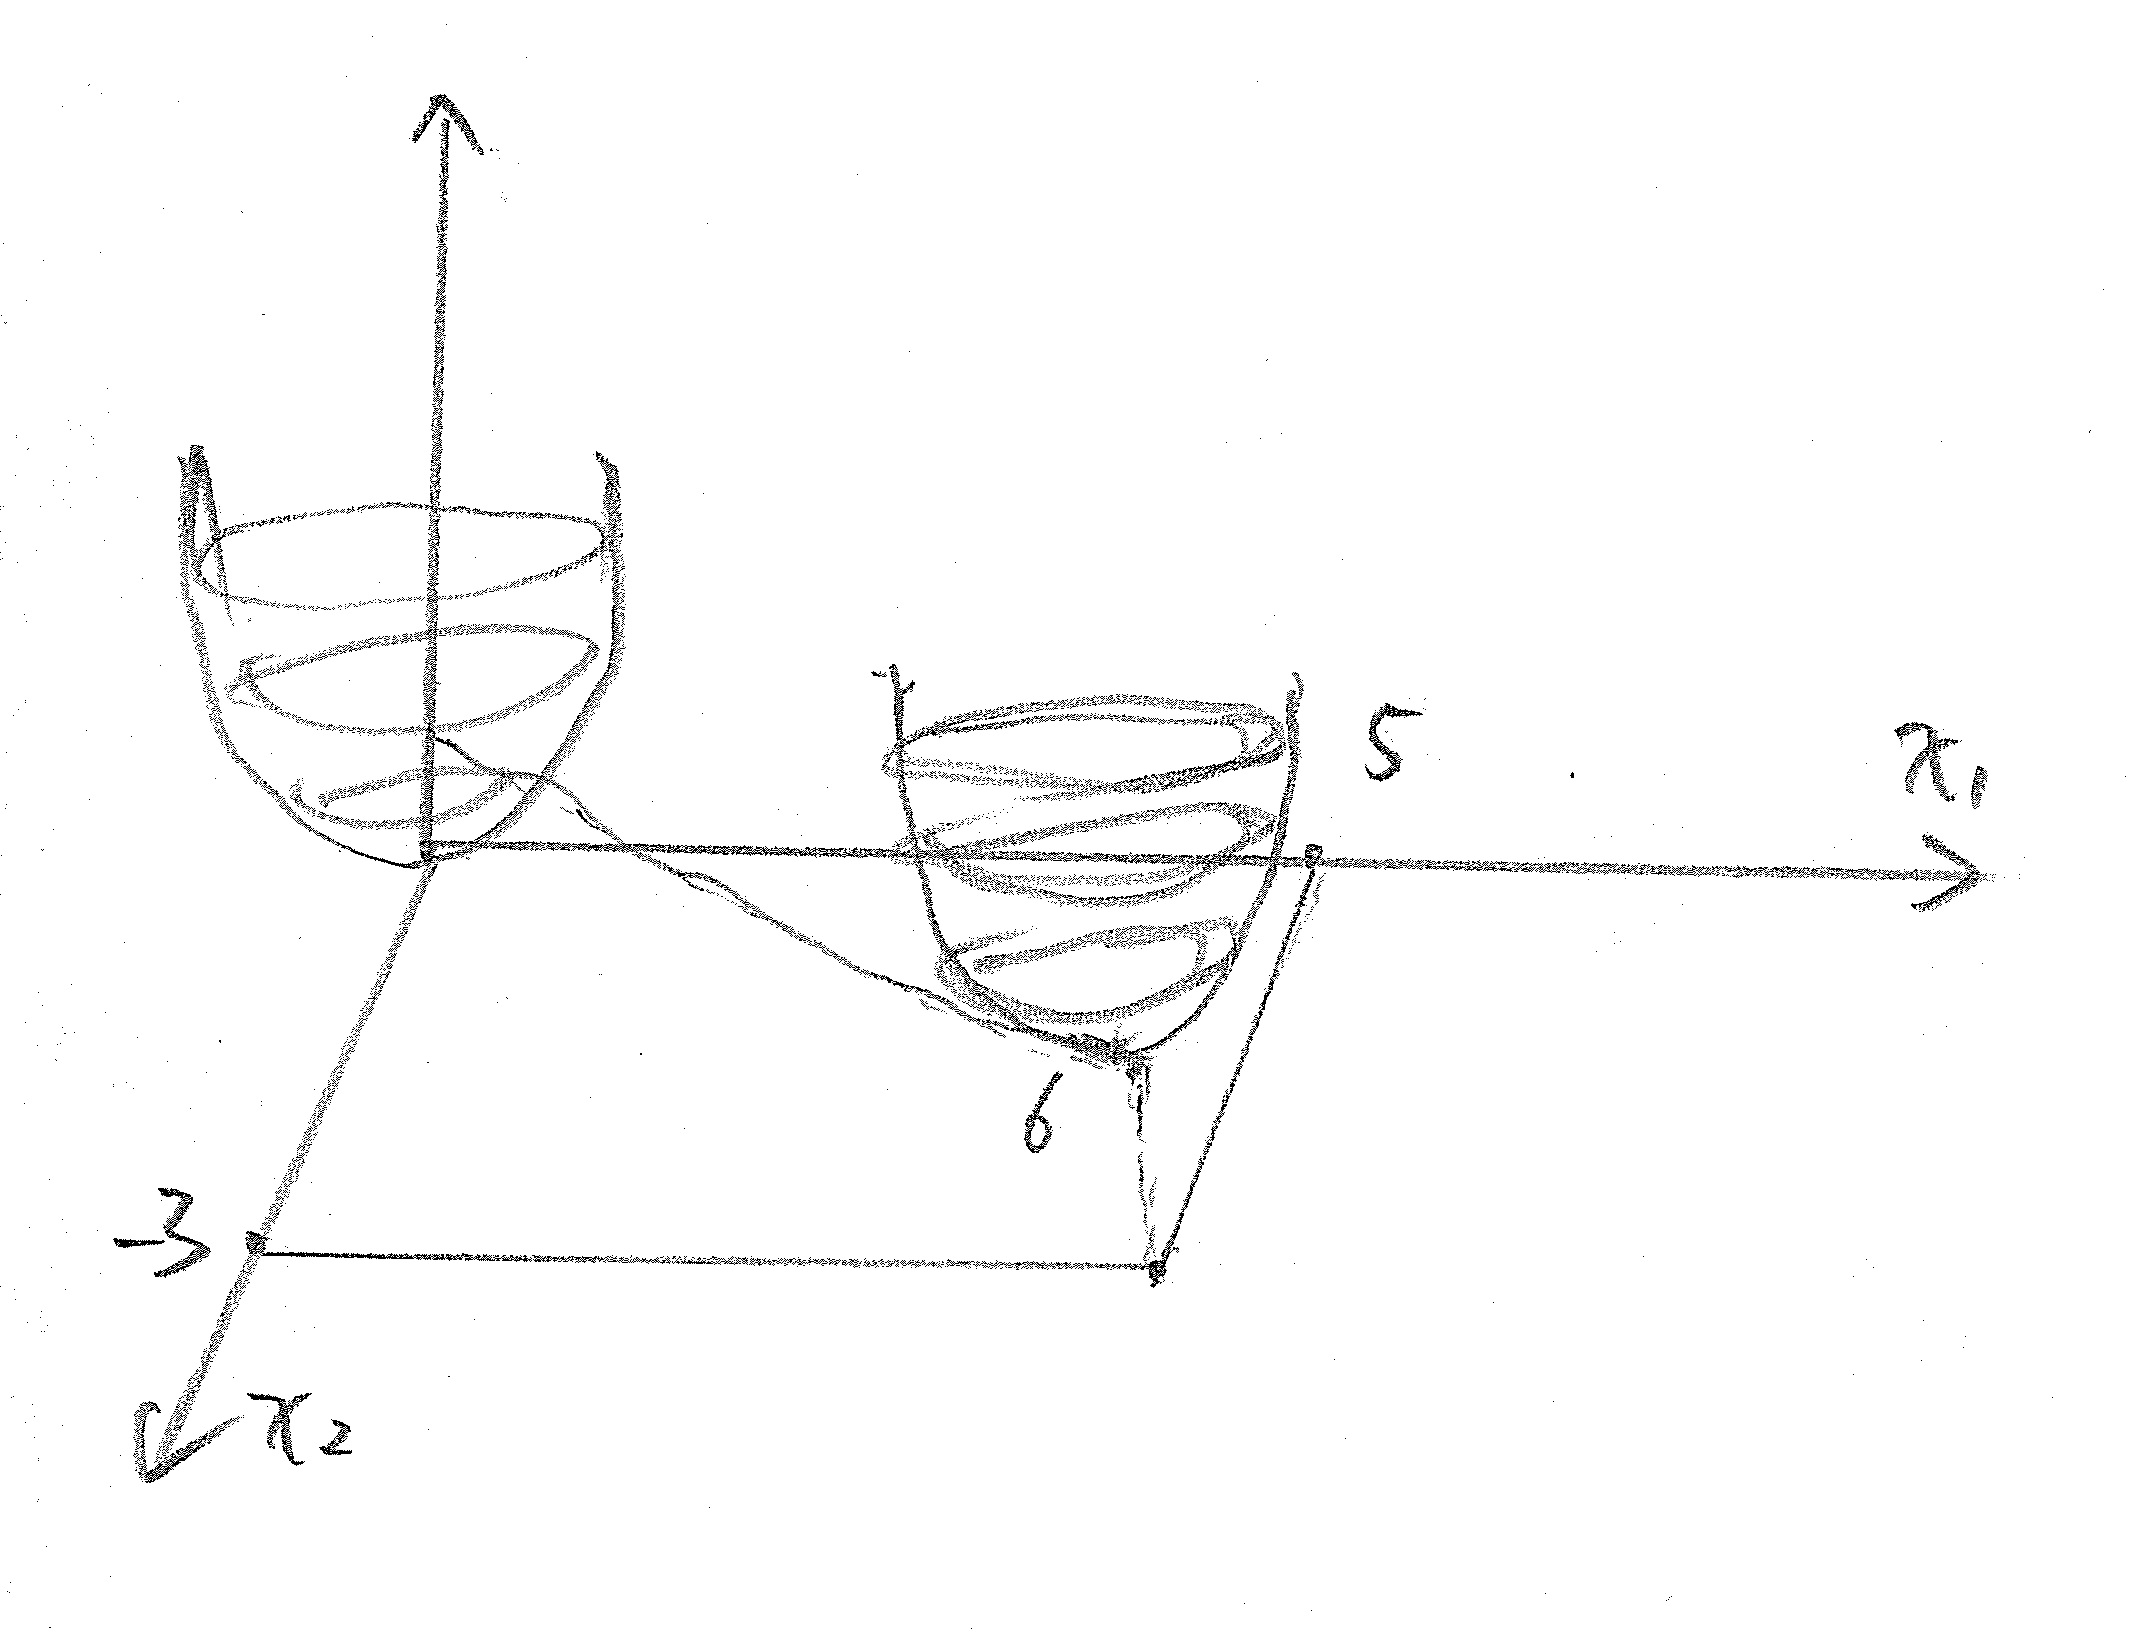
\includegraphics[width=1.8in,height=1.8in]{figures/ch06/ch06-06.jpg}
	%\caption{This is an inserted JPG graphic} 
	%\label{fig:graph} 
\end{figure}

\newpage
Draw level set for same picture
\begin{figure}
	\centering
	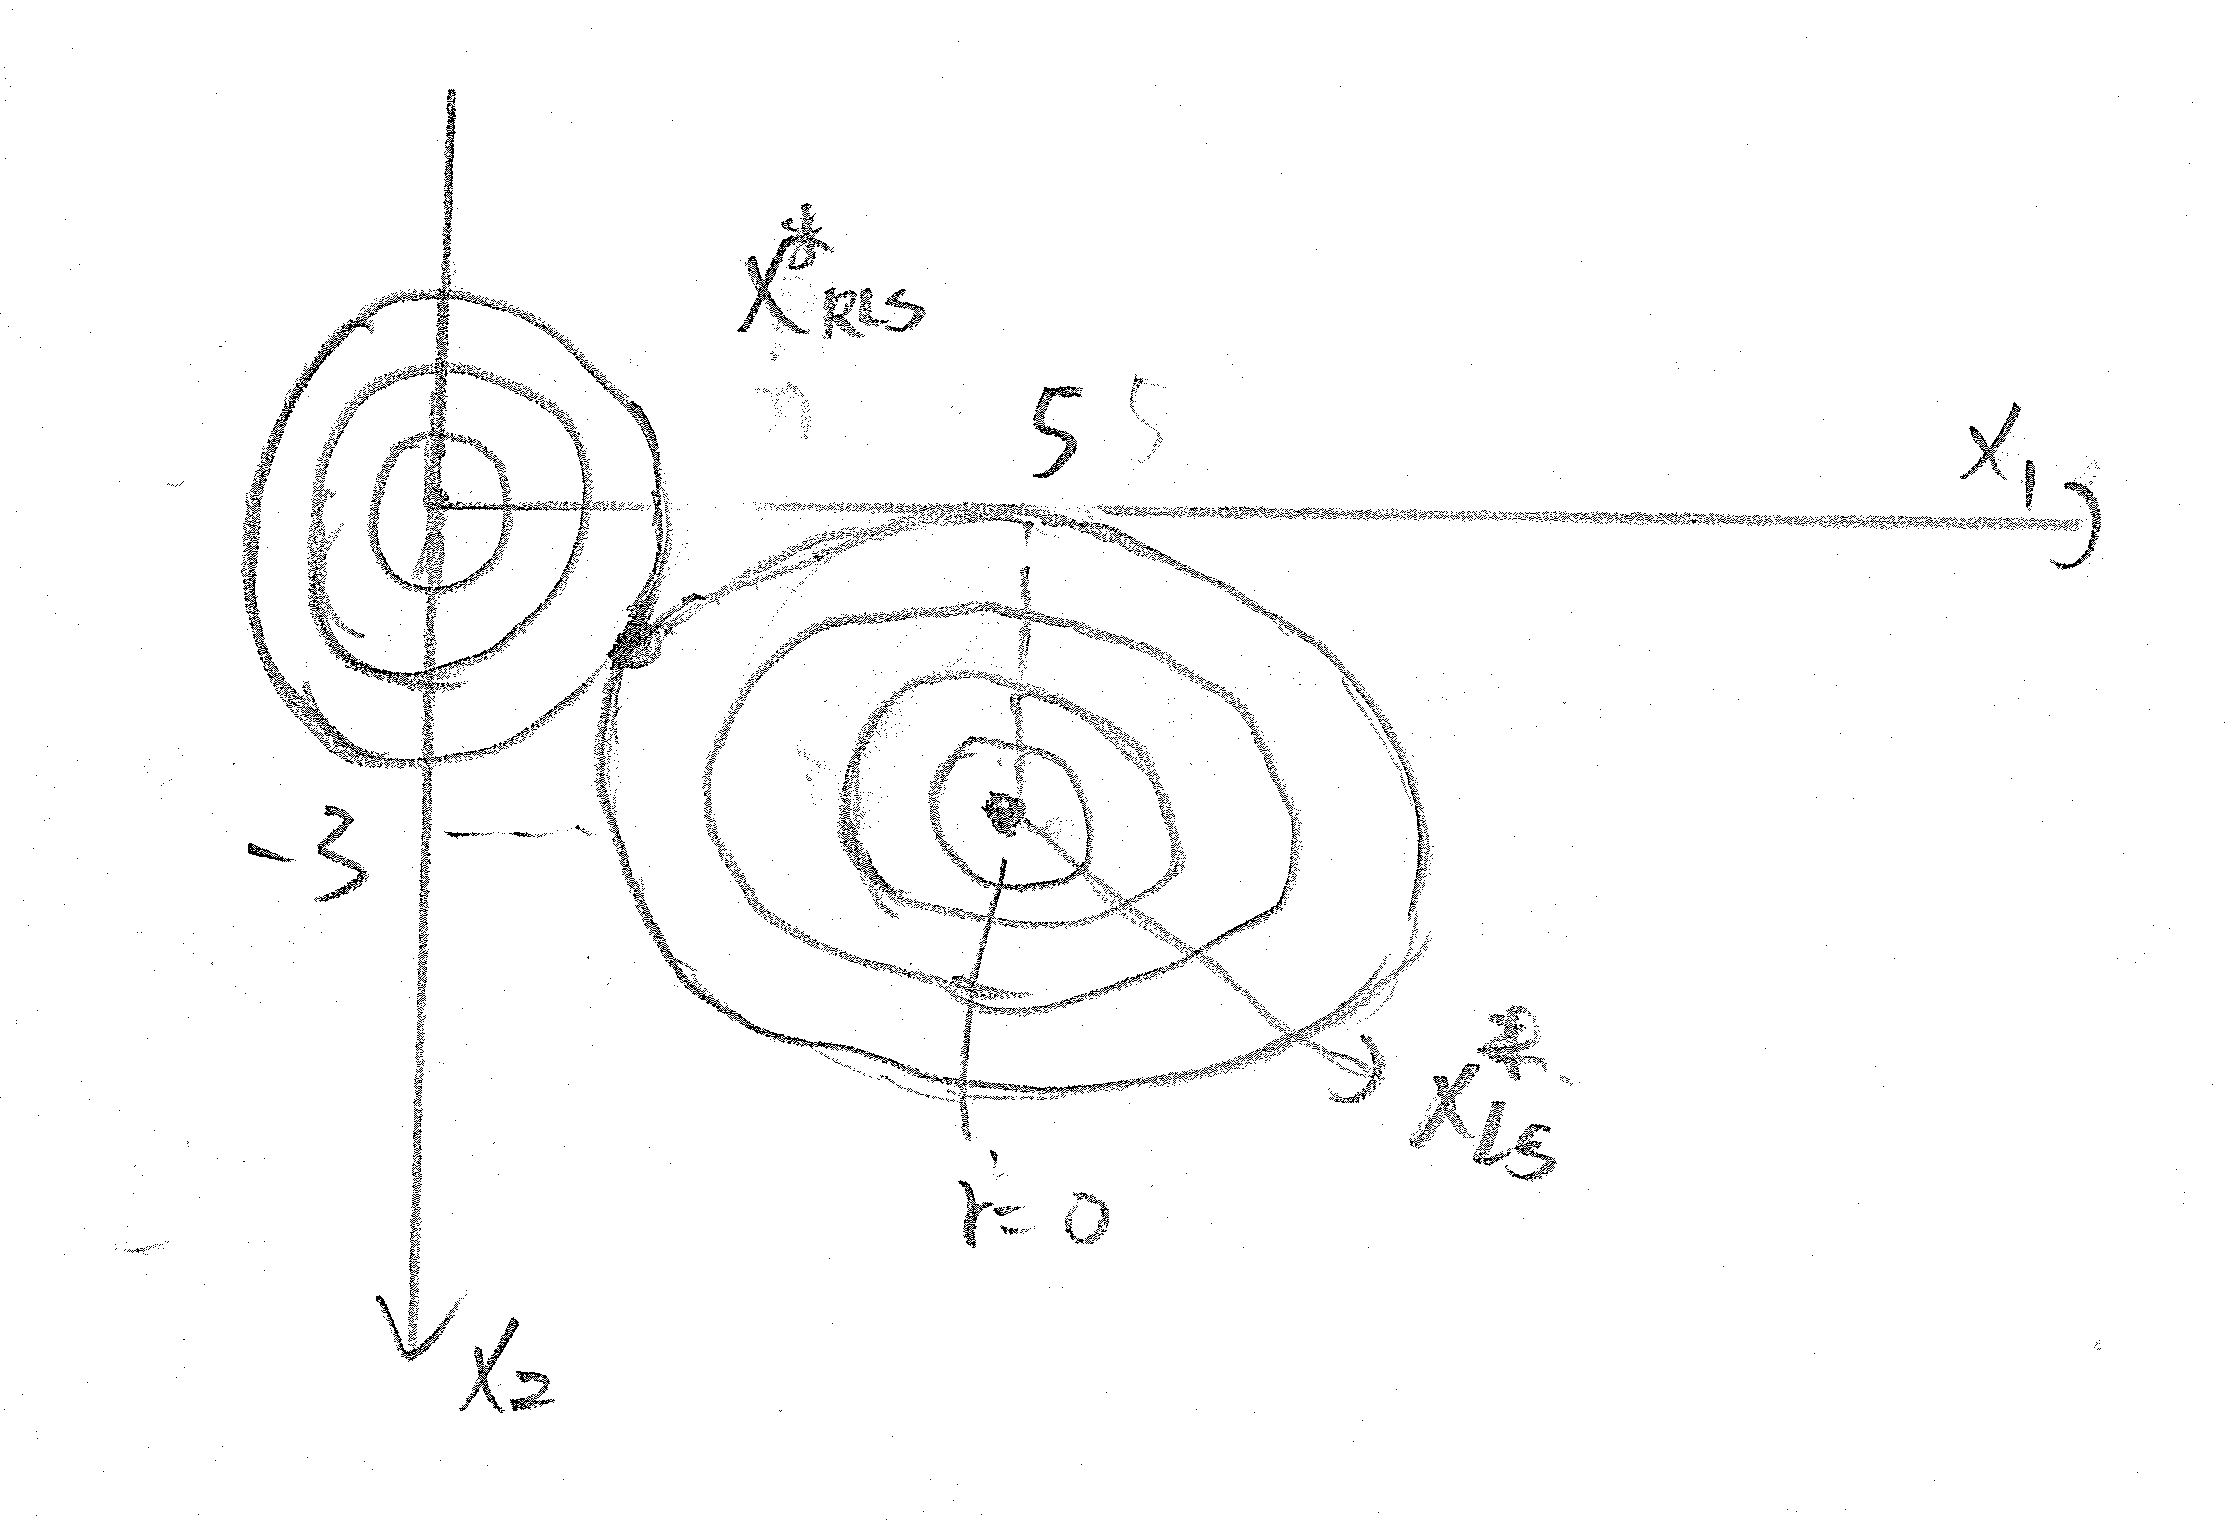
\includegraphics[width=1.8in,height=1.8in]{figures/ch06/ch06-07.jpg}
	%\caption{This is an inserted JPG graphic} 
	%\label{fig:graph} 
\end{figure}

\begin{align*}
c_1
&=\Vert Ax-y\Vert^2_2\\
&=\Vert A(x-x_{ls}^*+x_{ls}^*)-y\Vert^2_2\\
&=\Vert (Ax_{ls}^*-y)-A(x-x_{ls}^*)\Vert^2_2\\
&=\Vert (Ax_{ls}^*-y)\Vert^2_2 - \Vert A(x-x_{ls}^*)\Vert^2_2
\end{align*}

The first term on the last equality is a scalar 6(from previous example), and so we focus on the geometry of second term.
$$\Vert A(x-x_{ls}^*)\Vert^2_2= (x-x_{ls}^*)^{\trans} A^{\trans}A (x-x_{ls}^*)$$. 
Note that $A^{\trans}A$ is a PSD matrix. Understand geometry of level set of $\Vert A(x-x_{ls})\Vert^2_2$ via eigenvector of the PSD matrix $A^{\trans} A$

$$A^{\trans}A=
\begin{bmatrix}
3&3\\
3&5
\end{bmatrix}
=
\begin{bmatrix}
-0.81&0.58\\
058&0.81
\end{bmatrix}
\begin{bmatrix}
0.84&0\\
0&7.14
\end{bmatrix}
\begin{bmatrix}
-0.81&0.58\\
058&0.81
\end{bmatrix}
$$
\begin{marginfigure}
	\centering
	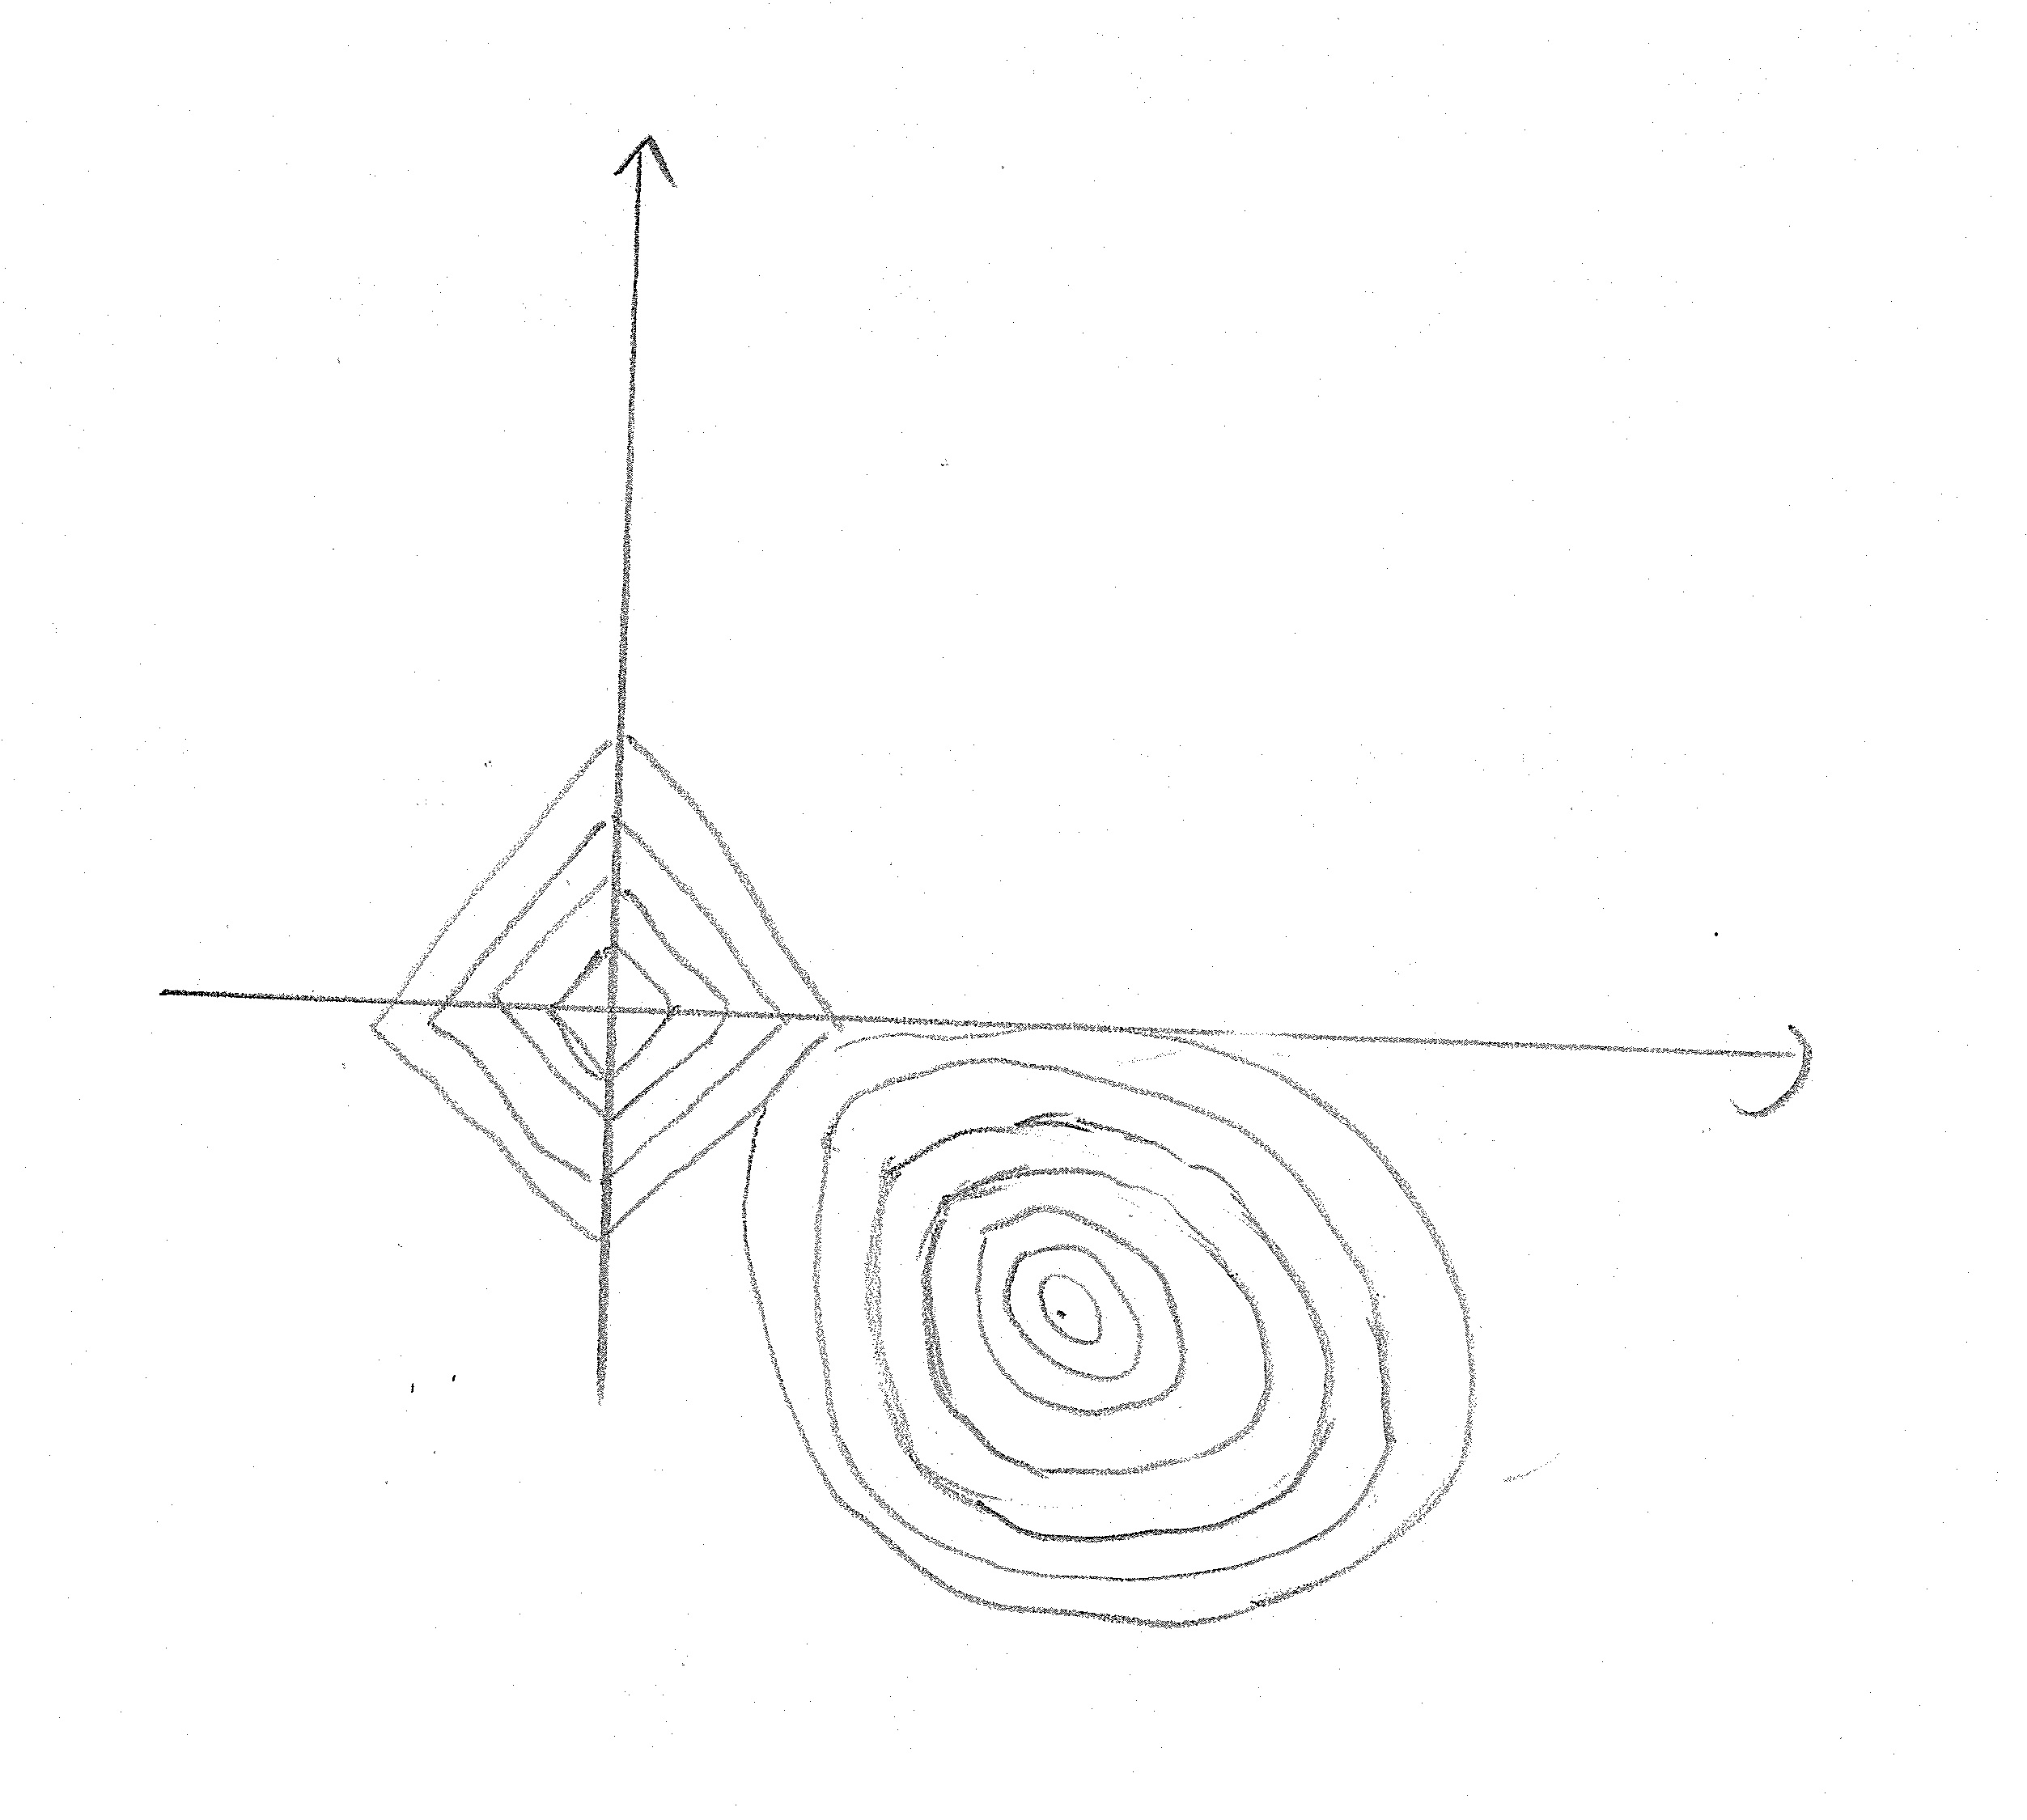
\includegraphics[width=1.8in,height=1.8in]{figures/ch06/ch06-08.jpg}
	%\caption{This is an inserted JPG graphic} 
	%\label{fig:graph} 
\end{marginfigure}


\subsection{Brief summary of Least Squares}
\begin{equation*}
x^* = \arg \min_{x\in \reals^n}\Vert y-Ax\Vert_2^2 \qquad (*)
\end{equation*}

	(1) Standard LS variant in ($*$) weights all elements of error vector equally (variant: weighted LS).
	
	(2) Standard LS measures error along standard coordinate system (change coordinate system).
	
	(3) Standard LS ignores that certain elements of $x$ may "cost" more than others (variant: regularization).

\subsection{More on "Tikhanov regularization"}
We do a simple example here, as a special case of "Tikhanov regularization, 
\begin{equation*}
x^* = \arg\min_{x\in \reals^n}\Vert y-Ax\Vert_2^2 + \gamma\Vert x\Vert_2^2
\end{equation*}

\begin{marginfigure}
	\centering
	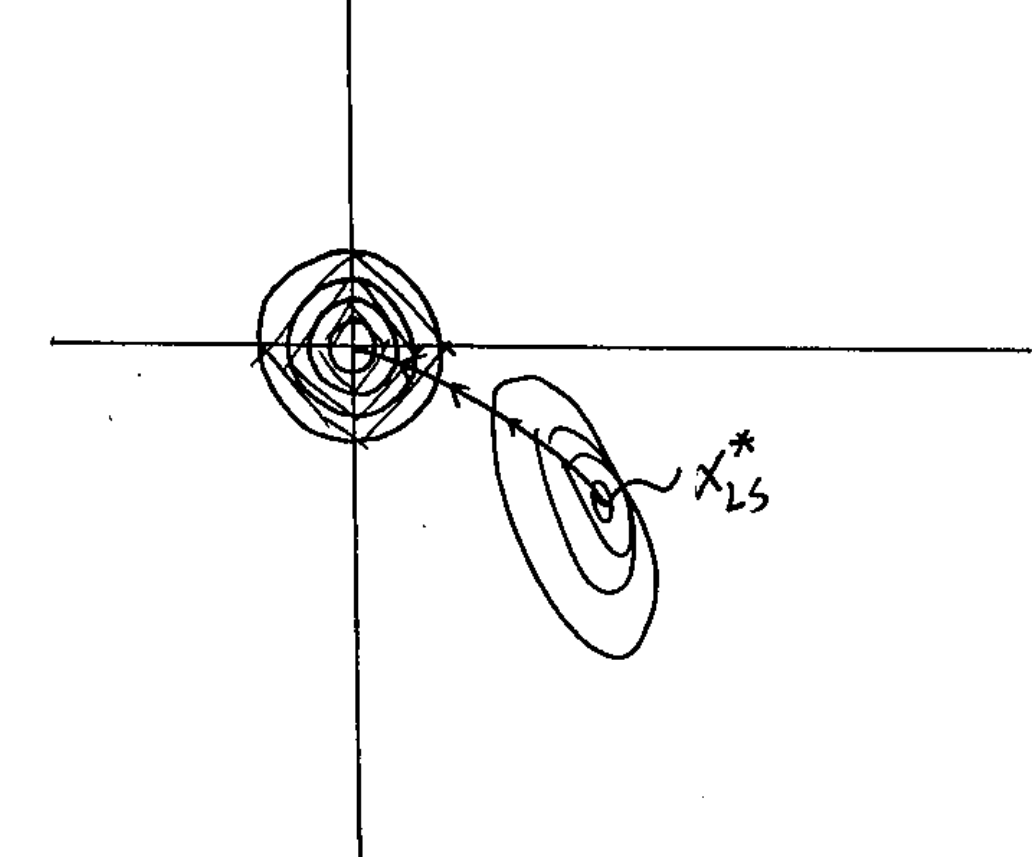
\includegraphics[width=1.8in,height=1.8in]{figures/ch06/figure4.png}
	%\caption{This is an inserted JPG graphic} 
	%\label{fig:graph} 
\end{marginfigure}

Look at the form of optimal solution 
\begin{align*}
x^* 
&= \arg\min_{x\in \reals^n}\Vert y-Ax\Vert_2^2 + \gamma\Vert x\Vert^2_2\\
&= (A^{\trans}A + \gamma I)^{-1}A^{\trans}y\\
\hat{y}^*&= Ax^* = A(A^{\trans}A + \gamma I)^{-1}A^{\trans}y\\
\end{align*}

We apply SVD to $A$,
$$A = \mathcal{U}\tilde{\Sigma}V^{\trans}$$

And utilize this to analyze $(A^{\trans}A + \gamma I)^{-1}$:
\begin{align*}
(A^{\trans}A + \gamma I)^{-1} 
&= (V\tilde{\Sigma}^{\trans}\mathcal{U}^{\trans}\mathcal{U}\tilde{\Sigma}V^{\trans} + \gamma I)^{-1}\\
&= (V
\begin{bmatrix}
\Sigma^{\trans} & 0\\
0 & 0\\
\end{bmatrix}
\begin{bmatrix}
\Sigma & 0\\
0 & 0\\
\end{bmatrix}
V^{\trans} + \gamma I)^{-1}\\
&=(V
\begin{bmatrix}
\Sigma^2 & 0\\
0  & 0
\end{bmatrix}
V^{\trans} + \gamma VV^{\trans}
)^{-1}\\
&= (V(
\begin{bmatrix}
\Sigma^2 & 0\\
0 & 0
\end{bmatrix}
+\gamma I)V^{\trans})^{-1}\\
&= V
\left[
\begin{array}{c|c}
\Sigma^2+\gamma I_r&  \\ \hline 
& \gamma I_{n-r}
\end{array}
\right]
V^{\trans}\\
&=
V
\left[
\begin{array}{c|c}
(\Sigma^2+\gamma I_r)^{-1}&  \\ \hline 
& ( \gamma I_{n-r})^{-1}
\end{array}
\right]
V^{\trans}\\
&=
V
\left[
\begin{array}{c|c}
\begin{matrix}
\frac{1}{\sigma_1^2+\gamma} & &\\
&\ddots&\\
&&\frac{1}{\sigma_r^2+\gamma}
\end{matrix}&  \\ \hline 
& \begin{matrix}
\frac{1}{\gamma} & &\\
&\ddots&\\
&&\frac{1}{\gamma}
\end{matrix}
\end{array}
\right]
V^{\trans}
\end{align*}

%\begin{matrix}
%	\frac{1}{\sigma_1^2+\gamma} & &\\
%	&...&\\
%	&&\frac{1}{\sigma_r^2+\gamma}
%\end{matrix}


%\left[
%\begin{array}{c|c}
%	\begin{matrix}
%		\frac{1}{\sigma_1^2+\gamma} & &\\
%		&...&\\
%		&&\frac{1}{\sigma_r^2+\gamma}
%	\end{matrix}&  \\ \hline 
%	& \begin{matrix}
%		\frac{1}{\gamma} & &\\
%		&...&\\
%		&&\frac{1}{\gamma}
%	\end{matrix}
%\end{array}
%\right]

\begin{align*}
y^* &= Ax^* = A(A^{\trans}A + \gamma I)^{-1}A^{\trans}y\\
&= \mathcal{U}\tilde{\Sigma}V^{\trans}\left(V
\left[
\begin{array}{c|c}
\begin{matrix}
\frac{1}{\sigma_1^2+\gamma} & &\\
&\ddots&\\
&&\frac{1}{\sigma_r^2+\gamma}
\end{matrix}&  \\ \hline 
& \begin{matrix}
\frac{1}{\gamma} & &\\
&\ddots&\\
&&\frac{1}{\gamma}
\end{matrix}
\end{array}
\right]
V^{\trans}\right)V\tilde{\Sigma}^{\trans}\mathcal{U}^{\trans}y\\
&= \mathcal{U}
\begin{bmatrix}
\Sigma & 0\\
0 & 0
\end{bmatrix}
\left[
\begin{array}{c|c}
\begin{matrix}
\frac{1}{\sigma_1^2+\gamma} & &\\
&\ddots&\\
&&\frac{1}{\sigma_r^2+\gamma}
\end{matrix}&  \\ \hline 
& \begin{matrix}
\frac{1}{\gamma} & &\\
&\ddots&\\
&&\frac{1}{\gamma}
\end{matrix}
\end{array}
\right]
\begin{bmatrix}
\Sigma^{\trans} & 0\\
0 & 0
\end{bmatrix}
\mathcal{U}^{\trans}y\\
&= \mathcal{U}
\left[
\begin{array}{c|c}
\begin{matrix}
\frac{\sigma_1^2}{\sigma_1^2+\gamma} & &\\
&\ddots&\\
&&\frac{\sigma_r^2}{\sigma_r^2+\gamma}
\end{matrix}&  \\ \hline 
& 0
\end{array}
\right]
\mathcal{U}^{\trans}y
\\
&= \mathcal{U}
\left[
\begin{array}{c|c}
\begin{matrix}
\frac{\sigma_1^2}{\sigma_1^2+\gamma} & &\\
&\ddots&\\
&&\frac{\sigma_r^2}{\sigma_r^2+\gamma}
\end{matrix}&  \\ \hline 
& 0
\end{array}
\right]
\begin{bmatrix}
\langle u^{(1)}, y\rangle\\
\langle u^{(2)}, y\rangle\\
\vdots\\
\langle u^{(m)}, y\rangle
\end{bmatrix}\\
&=\mathcal{U}
\begin{bmatrix}
\frac{\sigma_1^2}{\sigma_1^2+\gamma}\langle u^{(1)}, y\rangle\\
\vdots\\
\frac{\sigma_r^2}{\sigma_r^2+\gamma}\langle u^{(r)}, y\rangle\\
0\\
\vdots\\
0
\end{bmatrix}\\
&= \sum^r_{i=1}\frac{\sigma_i^2}{\sigma_i^2 + \gamma}\langle u^{(i)}, y\rangle u^{(i)}
\end{align*}

From the last equality,
\begin{equation*}
\sum^r_{i=1}\frac{\sigma_i^2}{\sigma_i^2 + \gamma}\langle u^{(i)}, y\rangle u^{(i)}
\end{equation*}

We should note that:
\begin{itemize}
	\item $\frac{\sigma_i^2}{\sigma_i^2 + \gamma}$: scaling is changed by regularization. If $\gamma = 0$, then  $\frac{\sigma_i^2}{\sigma_i^2 + \gamma} = 1$ and get back standard LS. If $\gamma > 0$, it's shrinkage. 
	
	\item $\langle u^{(i)}, y\rangle $: projection of data vector $y$ along that $i^{th}$ direction. 
	
	\item $u^{(i)}$: component of approximation along $i^{th}$ direction or $i^{th}$ basis element. 
\end{itemize}



